% This LaTeX was auto-generated from MATLAB code.
% To make changes, update the MATLAB code and export to LaTeX again.

\documentclass{article}

\usepackage[utf8]{inputenc}
\usepackage[T1]{fontenc}
\usepackage{lmodern}
\usepackage{graphicx}
\usepackage{color}
\usepackage{hyperref}
\usepackage{amsmath}
\usepackage{amsfonts}
\usepackage{epstopdf}
\usepackage[table]{xcolor}
\usepackage{matlab}

\sloppy
\epstopdfsetup{outdir=./}
\graphicspath{ {./submission_images/} }

\matlabhastoc

\begin{document}

\label{T_13326F55}
\matlabtitle{ECE1895 PROJECT1 REPORT}

\begin{par}
\begin{flushleft}
YINHAO | FALL2022 | ECE1895 | PROJECT1
\end{flushleft}
\end{par}

\matlabtableofcontents{Table of Contents}

\label{H_0F25CE15}
\matlabheading{1 Design Overview}

\label{H_CF48AC39}
\matlabheadingtwo{1.1 High Level Descriptions and Purposes}

\begin{par}
\begin{flushleft}
The 555 timer is omnipresent in our physical world. In ENGR1050 - Product Realization, our group is commisioned to refine the electronic Kesington Lock system, a lock connecting physical PCs or laptops with cables that alerts users of potential thief upon disconnections, hence a proposal to add an electronic alarming system that first buzz in lower frequency when connections with the protected device are unstable, a sign of potential tempering, and subsequently in higher frequency when connections are completely lost, a sign of confirmed tempering, is put forward. 
\end{flushleft}
\end{par}

\begin{par}
\begin{flushleft}
Indeed, The dual frequency buzzer can be implemented, along with some other trivial components, using a 555-timer and a simple mini speaker.
\end{flushleft}
\end{par}

\begin{par}
\begin{flushleft}
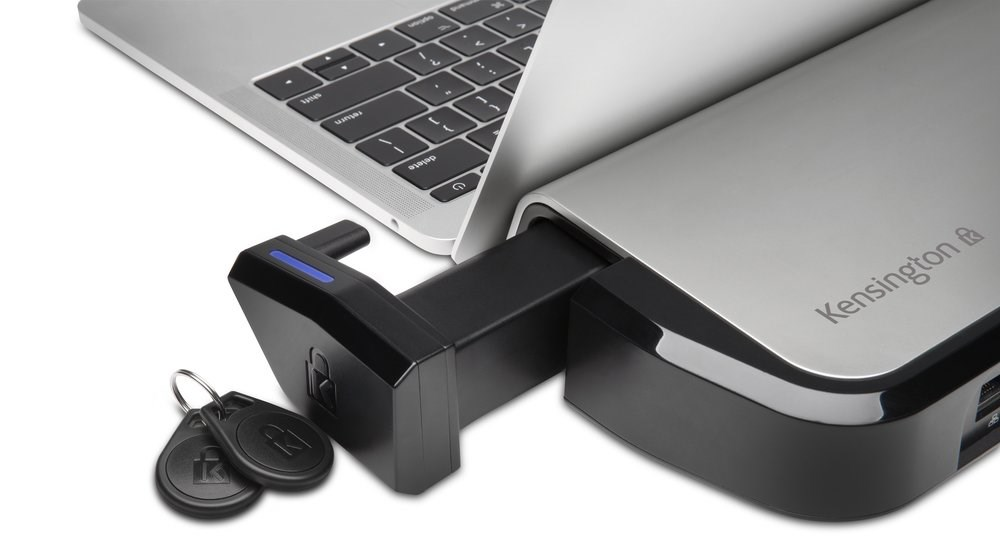
\includegraphics[width=\maxwidth{50.17561465127948em}]{image_0}
\end{flushleft}
\end{par}

\begin{par}
\begin{flushleft}
\textit{[Kensington Lock] }\href{https://www.kensington.com/news/security-blog/electronic-locking-technology-is-revolutionizing-device-security/}{\textit{https://www.kensington.com/news/security-blog/electronic-locking-technology-is-revolutionizing-device-security/}}
\end{flushleft}
\end{par}

\label{H_FA9851C9}
\matlabheadingtwo{1.2 Original Design}

\begin{par}
\begin{flushleft}
A simple buzzer design is found online from circuit-diy.com and will be referenced for this design. 
\end{flushleft}
\end{par}

\begin{par}
\begin{flushleft}
Below is the circuit schematic:
\end{flushleft}
\end{par}

\begin{par}
\begin{flushleft}
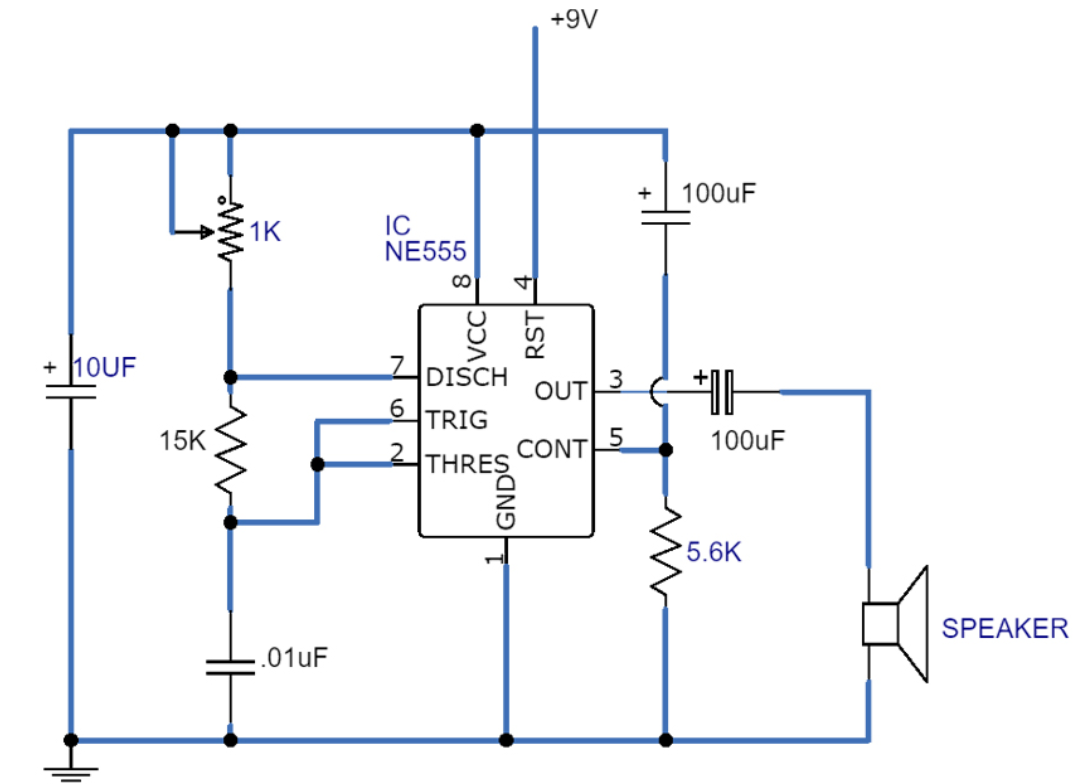
\includegraphics[width=\maxwidth{50.17561465127948em}]{image_1}
\end{flushleft}
\end{par}

\begin{par}
\begin{flushleft}
\textit{[Simple Buzzer Circuit] }\href{https://www.circuits-diy.com/simple-buzzer-circuit-with-ne555-ic/}{\textit{https://www.circuits-diy.com/simple-buzzer-circuit-with-ne555-ic/}}
\end{flushleft}
\end{par}

\begin{par}
\begin{flushleft}
The way how this circuit works is very simple: connect the +9V with our power supply, and the potentiometer will control the frequency in which the speaker will buzz.\textbf{ }
\end{flushleft}
\end{par}

\begin{par}
\begin{flushleft}
\textbf{However, there is one small mistake of this circuit diagram: the power supply should not only connects with RST but also with 10uF capacitor, 100uF capacitor on the top right, VCC form NE555, and the potentiometer. }
\end{flushleft}
\end{par}

\begin{par}
\begin{flushleft}
The fixed schematics should look something like this:
\end{flushleft}
\end{par}

\begin{par}
\begin{flushleft}
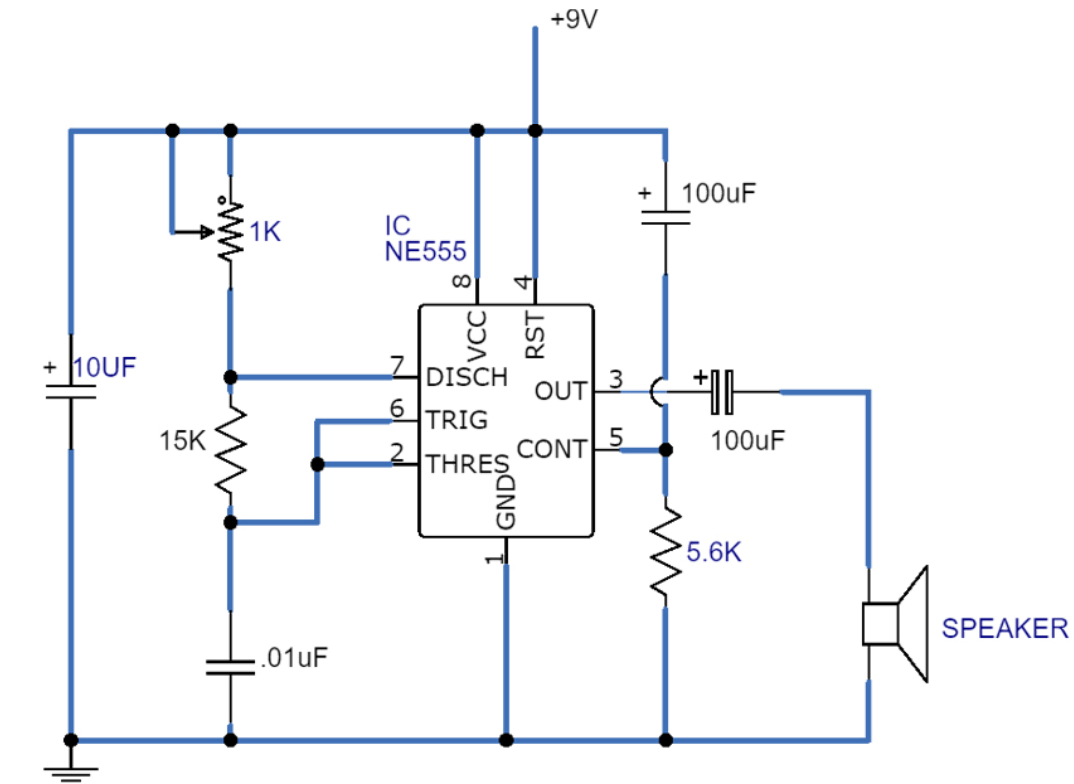
\includegraphics[width=\maxwidth{50.17561465127948em}]{image_2}
\end{flushleft}
\end{par}

\begin{par}
\begin{flushleft}
\textit{[Corrected Simple Buzzer Circuit]}
\end{flushleft}
\end{par}

\label{H_444C656C}
\matlabheadingtwo{1.3 Modifications and Improvements}

\begin{par}
\begin{flushleft}
The following changes are made comparing to the original design:
\end{flushleft}
\end{par}

\begin{enumerate}
\setlength{\itemsep}{-1ex}
   \item{\begin{flushleft} The 1K potentiometer is uncessary. Instread, we could use two resistors of fixed resistances, and each maps to one of the two frequencies. A two-way switch can be used to control which resistors the current will flow through. I will refer them as "control resistors pair" in this report. They are renamed to $R_{\textrm{HIGH}}$ and $R_{\textrm{LOW}}$ respectively, and their values will be calculated later. \end{flushleft}}
   \item{\begin{flushleft} Since the CONT(CV) pin is used to control the timing of the 555-timer by overriding the two-third VCC level from the voltage divider network, we could eliminate the 5.6K resistor on the bottom right and 100uF capacitor on the top right, since no overriding is needed after we finalize the resistances of control resistors pair, because they always result in a stable and desired state so long as the right values of resistances are carefully calculated and verified. CONT(CV) pin will now be hanging. \end{flushleft}}
   \item{\begin{flushleft} The low-pass filter capacitor is renamed to $\textrm{C1}$ , the multiplier capacitor to $\textrm{C2}$, and the second resistor in to $\textrm{R1}$. Their corresponding values will be calculated later.  \end{flushleft}}
   \item{\begin{flushleft} For versatility purposes, the voltage supply limitation being 9 volts is lifted as any would functionally power the circuit as long as within components' maximum limit. \end{flushleft}}
\end{enumerate}

\begin{par}
\begin{flushleft}
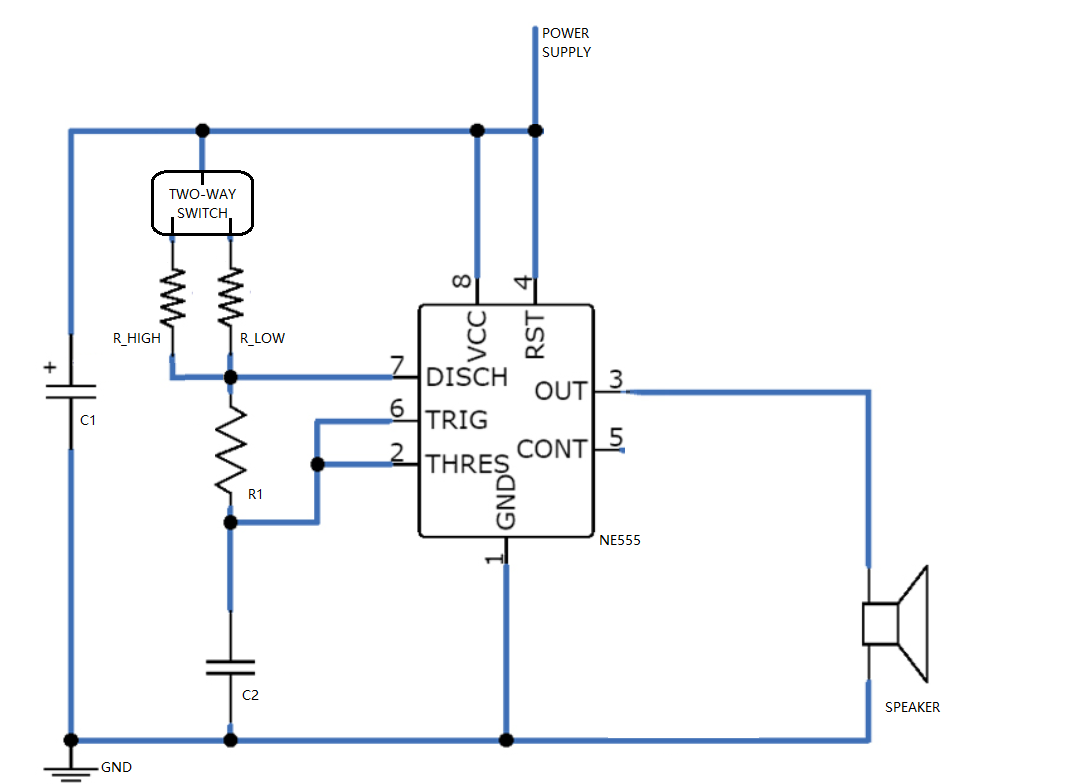
\includegraphics[width=\maxwidth{50.17561465127948em}]{image_3}
\end{flushleft}
\end{par}

\begin{par}
\begin{flushleft}
\textit{[Modified and Generalized Simple Buzzer Circuit]}
\end{flushleft}
\end{par}

\label{H_C294E082}
\matlabheadingtwo{1.4 Circuit Operations and Components Significances}

\begin{par}
\begin{flushleft}
To use this system, simply connect the power supply and ground, the alarm should immediately will be audible. The tone depends on the current state of the two-pin switch, and toggling the switch will change the tone accordingly. 
\end{flushleft}
\end{par}

\begin{par}
\begin{flushleft}
All compoents are essential for the circuit to function and cannot be removed:
\end{flushleft}
\end{par}

\begin{itemize}
\setlength{\itemsep}{-1ex}
   \item{\begin{flushleft} Power Supply: $\textrm{VCC}$- Supply the circuit with neccessary electric energy. \end{flushleft}}
   \item{\begin{flushleft} Low Pass Filter $\textrm{C1}$- This capacitor is able to make sure the voltage supplied to the 555-timer is stable when variations are present in the power supply. \end{flushleft}}
   \item{\begin{flushleft} Ground: $\textrm{GND}$ - Grounding the circuit so that a closed-loop is formed in order for the electrons to flow through the circuit.  \end{flushleft}}
   \item{\begin{flushleft} Two-way Switch: $\textrm{TWS}$ - It selects which resistor among $R_{\textrm{HIGH}}$ and $R_{\textrm{LOW}}$ the current will pass through, determining the tone of alarm. \end{flushleft}}
   \item{\begin{flushleft} Control Resistors Pair (First Resistor in Voltage Divider): $R_{\textrm{HIGH}}$ and $R_{\textrm{LOW}}$ - When one of the two is selected, they will predict the frequencies of the output signal from the 555-timer along with $\textrm{R1}$ and $\textrm{C2}$, and the time high along with $\textrm{R1}$ and $\textrm{C2}$. \end{flushleft}}
   \item{\begin{flushleft} Second Resistor in Voltage Divider $\textrm{R1}$- It will predict the frequencies and time low of the output signal from the 555-timer along with control resistors pair and $\textrm{C2}$, the time high along with Control Resistors Pair and $\textrm{C2}$. \end{flushleft}}
   \item{\begin{flushleft} Multiplier Capactor $\textrm{C2}$ - This capacitor will predict the frequencies and time low of the output signal from the 555-timer along with $\textrm{R1}$ and Control Resistors Pair, the time high along with $\textrm{R1}$ and Control Resistors Pair. \end{flushleft}}
   \item{\begin{flushleft} 555 Timer: $\textrm{NE555}$ - This will acts as \textbf{ASTABLE VIBORATOR }so that the speaker is able to make the buzzing sound.  \end{flushleft}}
\end{itemize}

\begin{par}
\begin{flushleft}
Their relationships can be generalized when the 555-timer is operating in the astable viborating mode:
\end{flushleft}
\end{par}

\begin{itemize}
\setlength{\itemsep}{-1ex}
   \item{\begin{flushleft} Time high: $T_{\textrm{HIGH}} =\left(0\ldotp 693\right)*\left(\textrm{TWS}?R_{\textrm{HIGH}} :R_{\textrm{LOW}} +\textrm{R1}\right)*\textrm{C2}$ \end{flushleft}}
   \item{\begin{flushleft} Time low: $T_{\textrm{LOW}} =\left(0\ldotp 693\right)*\textrm{R1}*\textrm{C2}$ \end{flushleft}}
   \item{\begin{flushleft} Frequency: $f=\frac{\left(1\ldotp 44\right)}{\left(\textrm{TWS}?R_{\textrm{HIGH}} :R_{\textrm{LOW}} +2*\textrm{R1}\right)*\textrm{C2}}$ \end{flushleft}}
\end{itemize}

\begin{par}
\begin{flushleft}
To acquire the approriate resistances and capacitances, we shall look at the datasheet of the speaker:
\end{flushleft}
\end{par}

\begin{par}
\begin{flushleft}
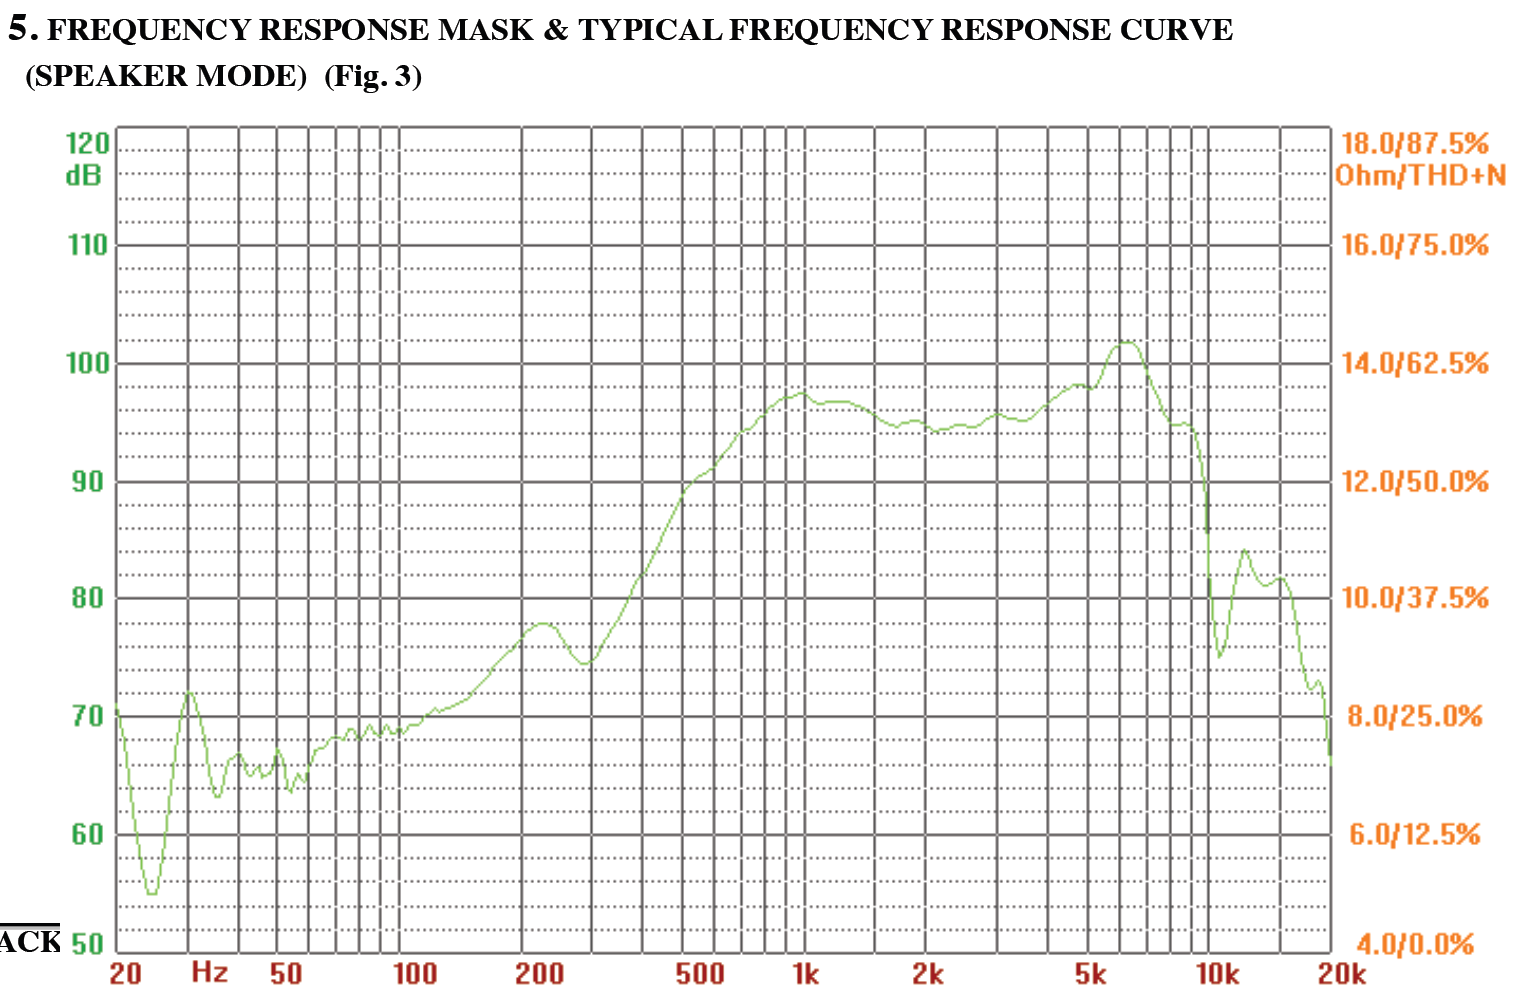
\includegraphics[width=\maxwidth{50.17561465127948em}]{image_4}
\end{flushleft}
\end{par}

\begin{par}
\begin{flushleft}
\textit{[Frequency Response of Speaker] }\href{https://www.sparkfun.com/products/9151}{\textit{https://www.sparkfun.com/products/9151}}
\end{flushleft}
\end{par}

\begin{par}
\begin{flushleft}
With this information on frequency range, all resistances and capacitances are able to be acquired via 555-Timer Calculator from Digikey:
\end{flushleft}
\end{par}

\begin{par}
\begin{flushleft}
\textbf{State 1 - High Frequency/Low Resistance Mode}
\end{flushleft}
\end{par}

\begin{par}
\begin{flushleft}
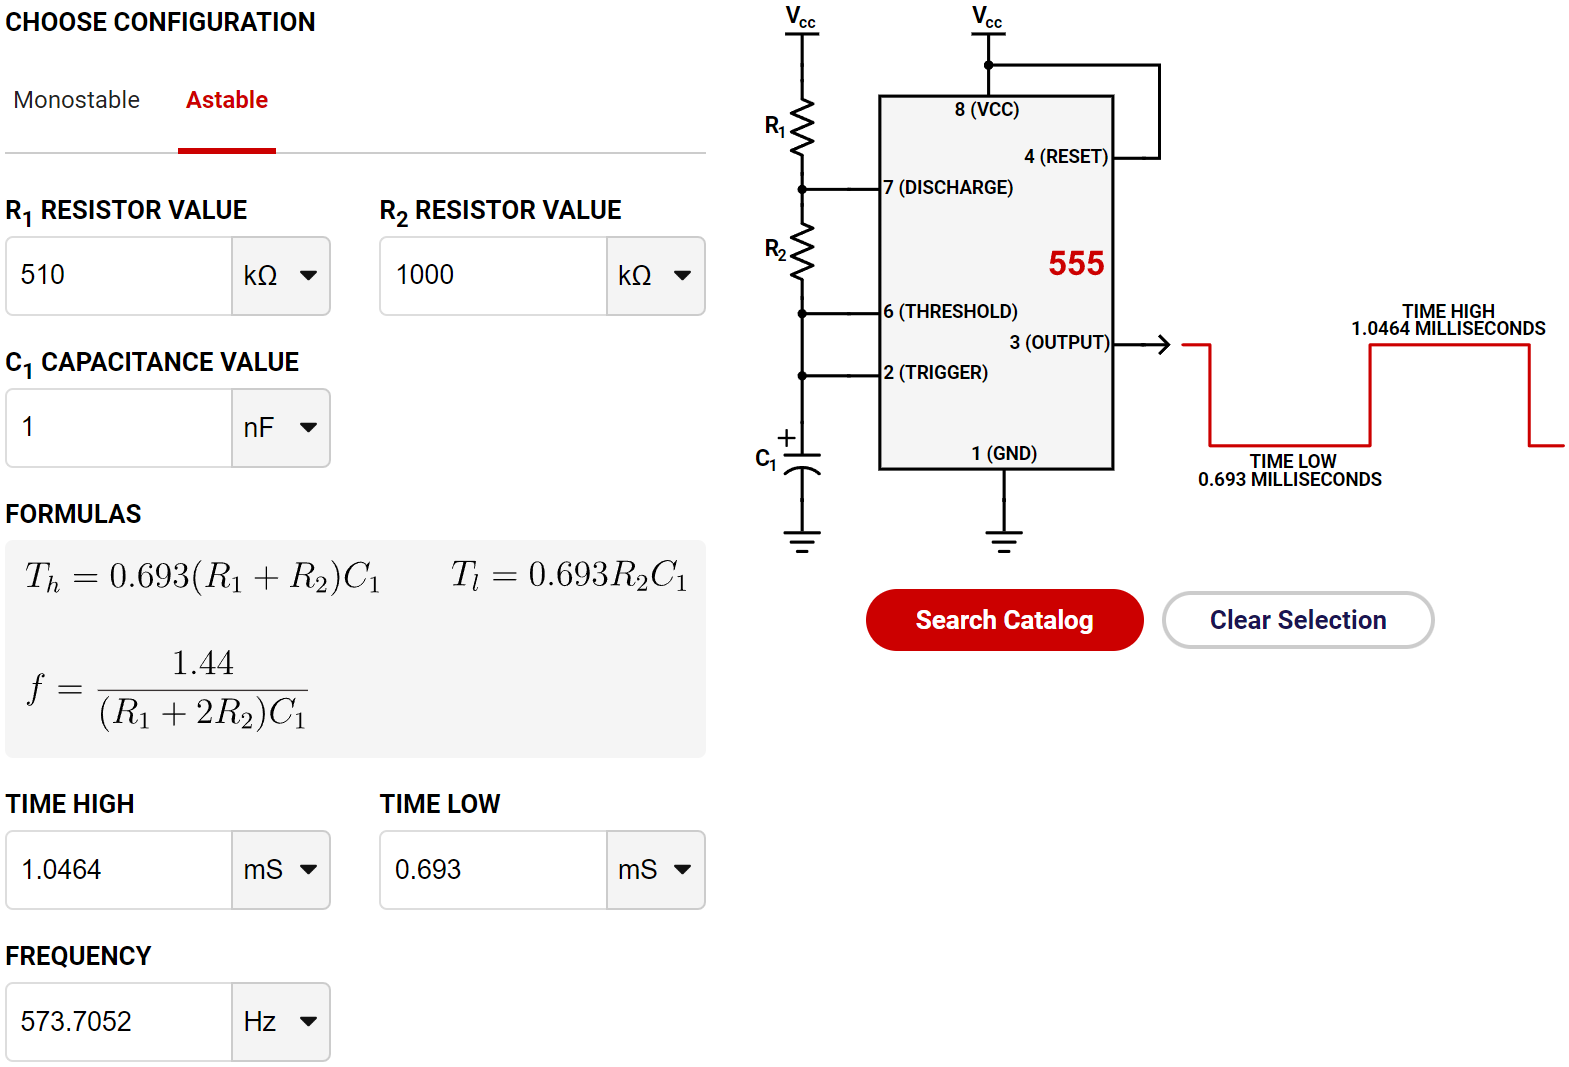
\includegraphics[width=\maxwidth{50.17561465127948em}]{image_5}
\end{flushleft}
\end{par}

\begin{par}
\begin{flushleft}
\textit{[555 Timer Calculator - Low Frequency Mode] }\href{https://www.digikey.com/en/resources/conversion-calculators/conversion-calculator-555-timer}{\textit{https://www.digikey.com/en/resources/conversion-calculators/conversion-calculator-555-timer}}
\end{flushleft}
\end{par}

\begin{par}
\begin{flushleft}
\textbf{State 2 - Low Frequency/High Resistance Mode}
\end{flushleft}
\end{par}

\begin{par}
\begin{flushleft}
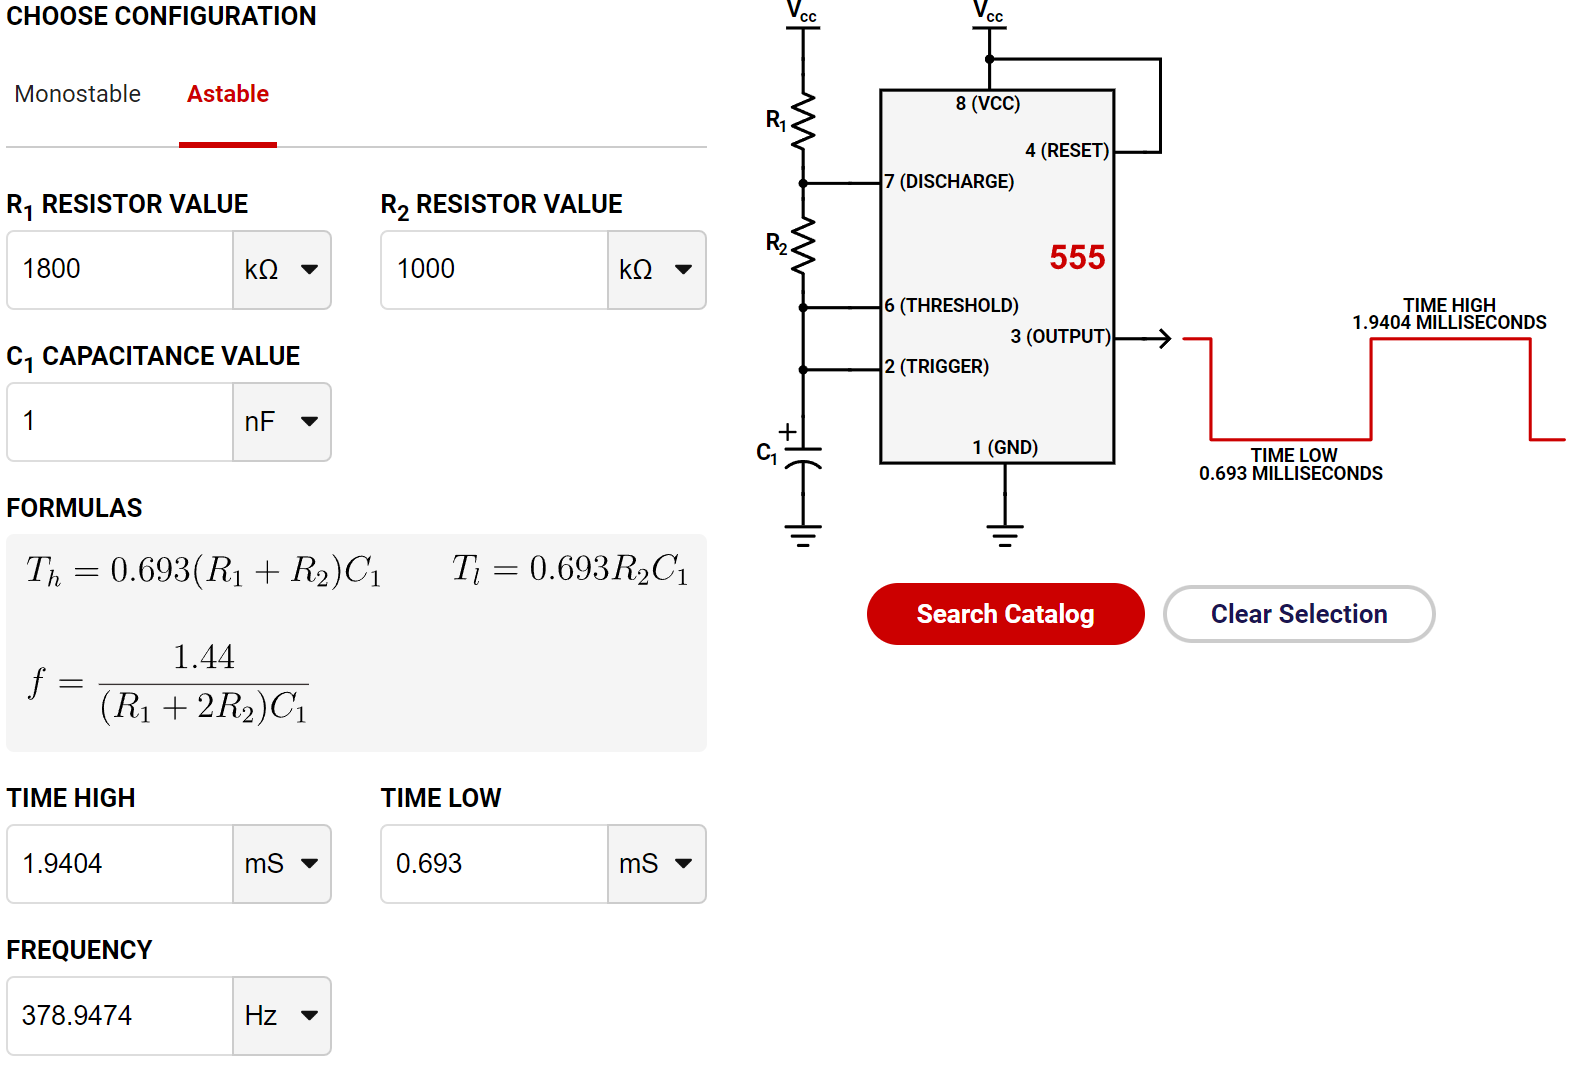
\includegraphics[width=\maxwidth{50.17561465127948em}]{image_6}
\end{flushleft}
\end{par}

\begin{par}
\begin{flushleft}
\textit{[555 Timer Calculator - High Frequency Mode] }\href{https://www.digikey.com/en/resources/conversion-calculators/conversion-calculator-555-timer}{\textit{https://www.digikey.com/en/resources/conversion-calculators/conversion-calculator-555-timer}}
\end{flushleft}
\end{par}

\begin{par}
\begin{flushleft}
With the following combinations, we are able to generate two audible frequencies with the following parameters:
\end{flushleft}
\end{par}

\begin{par}
$$\begin{array}{l}
R_{\textrm{LOW}} =510k\;\Omega \\
R_{\textrm{HIGH}} =1800k\Omega \\
\textrm{C2}=1\textrm{nF}
\end{array}$$
\end{par}

\begin{par}
\begin{flushleft}
For the low pass filter, a common capacitance is used:
\end{flushleft}
\end{par}

\begin{par}
$$\textrm{C1}=1\mu F$$
\end{par}


\label{H_7154AFCB}
\matlabheading{2 Design Verifications}

\label{H_50B7CA2B}
\matlabheadingtwo{2.1 Spice Verifications}

\label{H_15E11B9E}
\matlabheadingthree{2.1.1 Simulation Schematics:}

\begin{par}
\begin{flushleft}
Since it is not trivial to simulate the two-way switch in LTSpice, two modes of operation are each simulated.
\end{flushleft}
\end{par}

\begin{par}
\begin{flushleft}
Apart from the mentioned nuances, the remaining circuitray remains unchanged and then is simulated while the voltage for speaker input port for speaker is being observed: 
\end{flushleft}
\end{par}

\begin{par}
\begin{flushleft}
\textbf{State 1 - High Frequency/Low Resistance Mode}
\end{flushleft}
\end{par}

\begin{par}
\begin{flushleft}
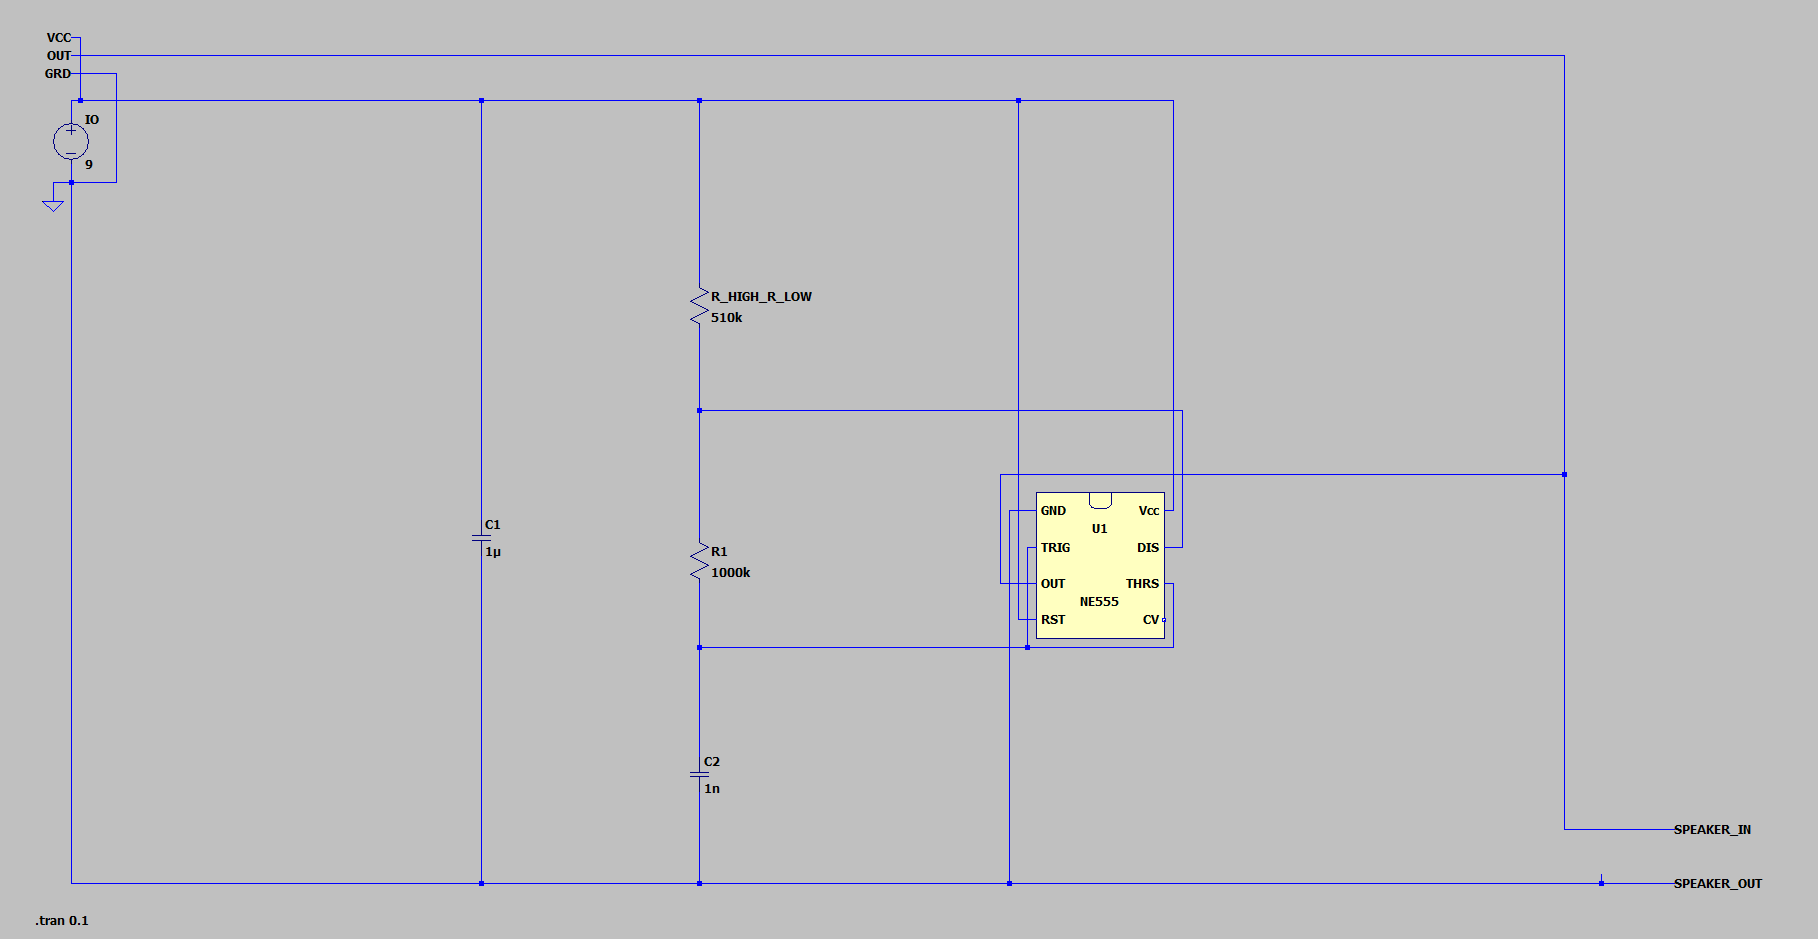
\includegraphics[width=\maxwidth{50.17561465127948em}]{image_7}
\end{flushleft}
\end{par}

\begin{par}
\begin{flushleft}
\textit{[LTSpice Schematics for State 1]}
\end{flushleft}
\end{par}

\begin{par}
\begin{flushleft}
\textbf{State 2 - Low Frequency/High Resistance Mode}
\end{flushleft}
\end{par}

\begin{par}
\begin{flushleft}
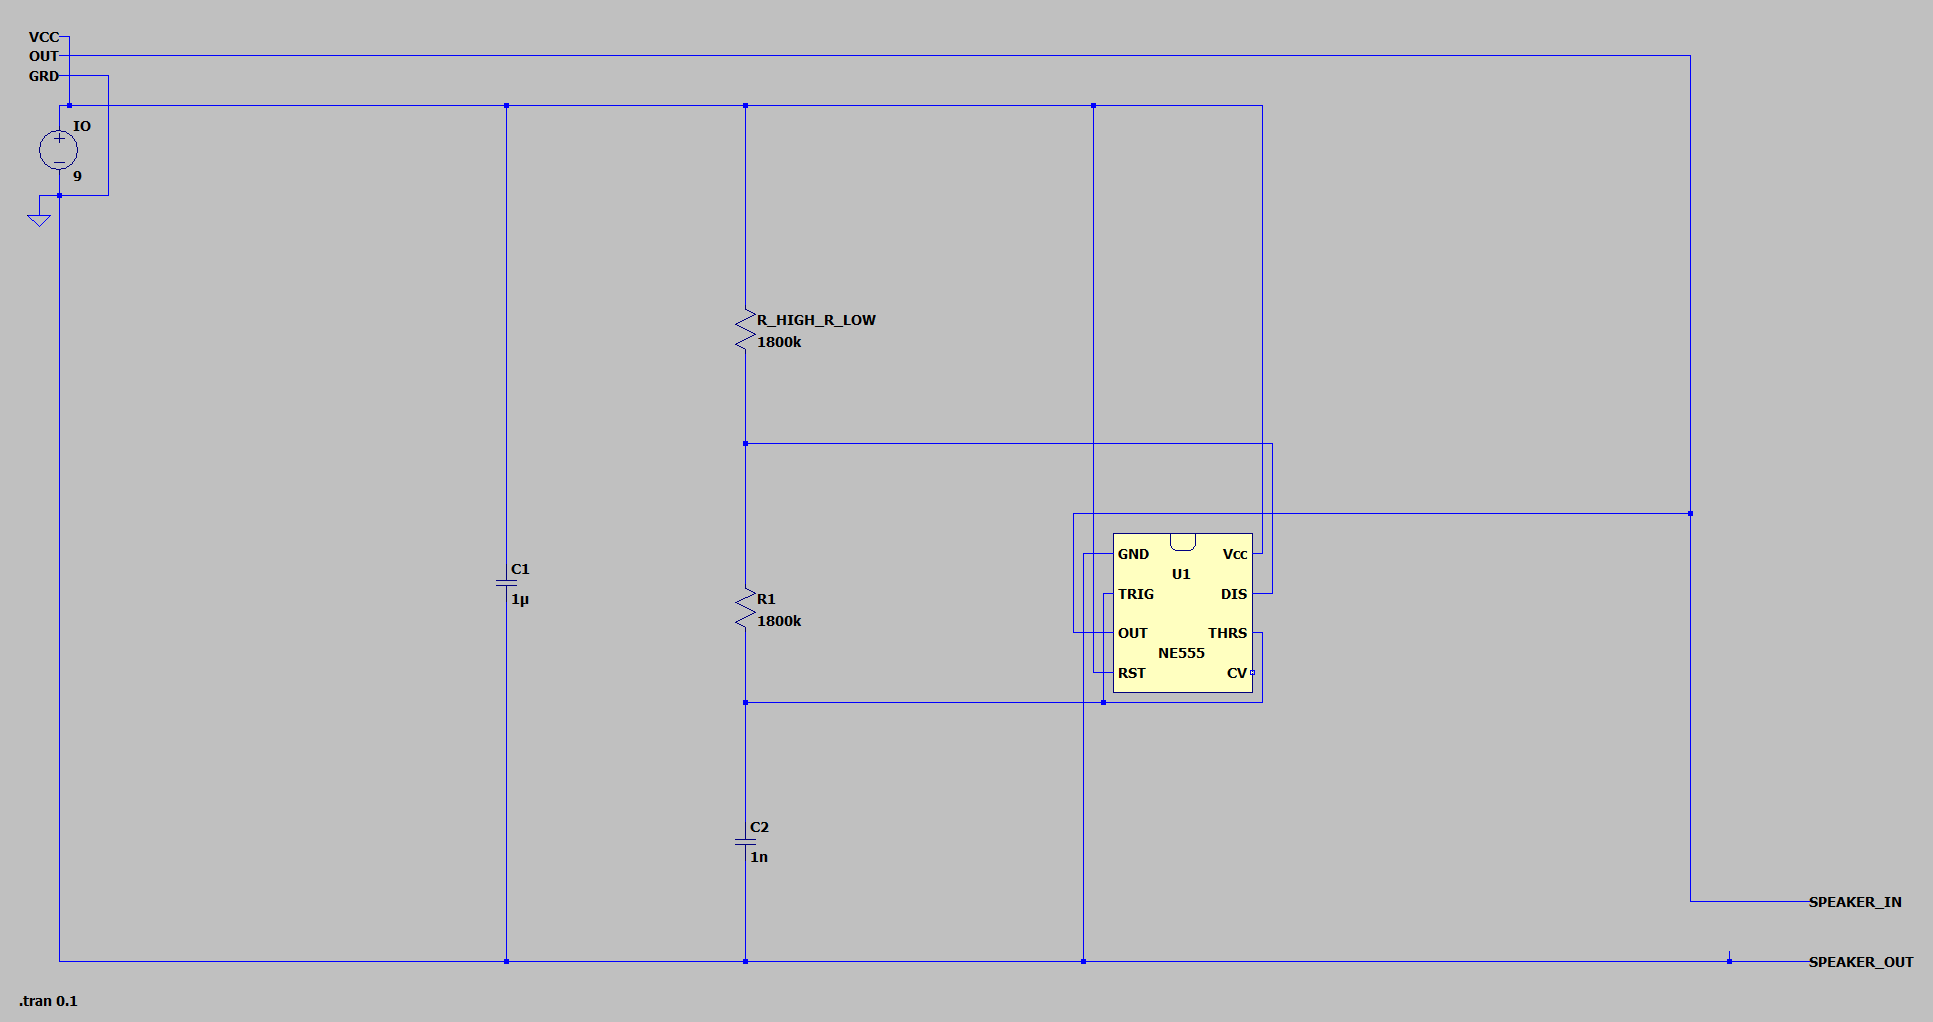
\includegraphics[width=\maxwidth{50.17561465127948em}]{image_8}
\end{flushleft}
\end{par}

\begin{par}
\begin{flushleft}
\textit{[LTSpice Schematics for State 2]}
\end{flushleft}
\end{par}

\label{H_D7A81969}
\matlabheadingthree{2.1.2 Creative Ways of Modelling}

\begin{par}
\begin{flushleft}
Since all components used in the design exist in PSpice library, there is no need for creative ways of modelling.
\end{flushleft}
\end{par}

\label{H_ED0BE591}
\matlabheadingthree{2.1.3 Simulation Parameters}

\begin{par}
\begin{flushleft}
Since the frequencies are \textasciitilde{}436 to \textasciitilde{}570 Hz, 100 miliseconds of transient simulation should be able to yield a observable output waveforms: 
\end{flushleft}
\end{par}

\begin{par}
\begin{flushleft}
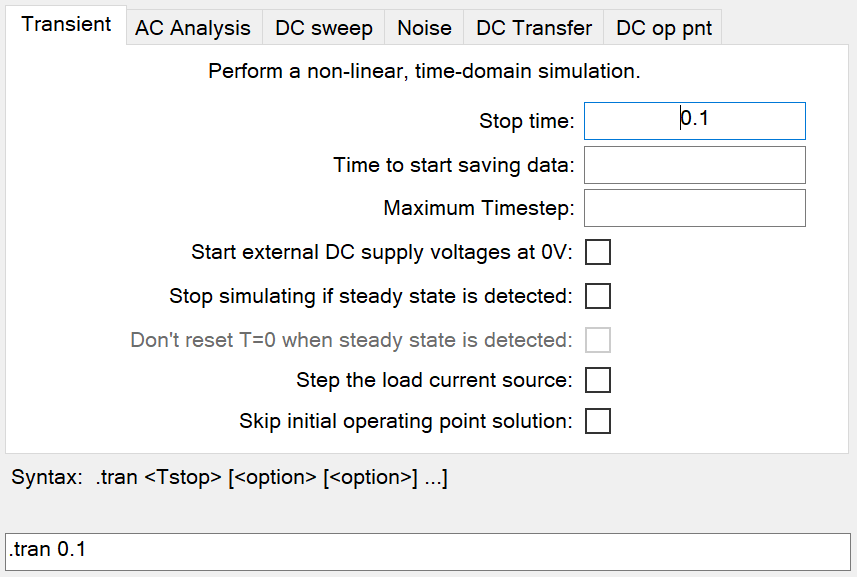
\includegraphics[width=\maxwidth{50.17561465127948em}]{image_9}
\end{flushleft}
\end{par}

\begin{par}
\begin{flushleft}
\textit{[LTSpice Parameters]}
\end{flushleft}
\end{par}

\label{H_90DA6073}
\matlabheadingthree{2.1.4 Simulation Results and Waveforms}

\begin{par}
\begin{flushleft}
After running the the simulations, resulted waveforms indicate that the design is legitimate: 
\end{flushleft}
\end{par}

\begin{par}
\begin{flushleft}
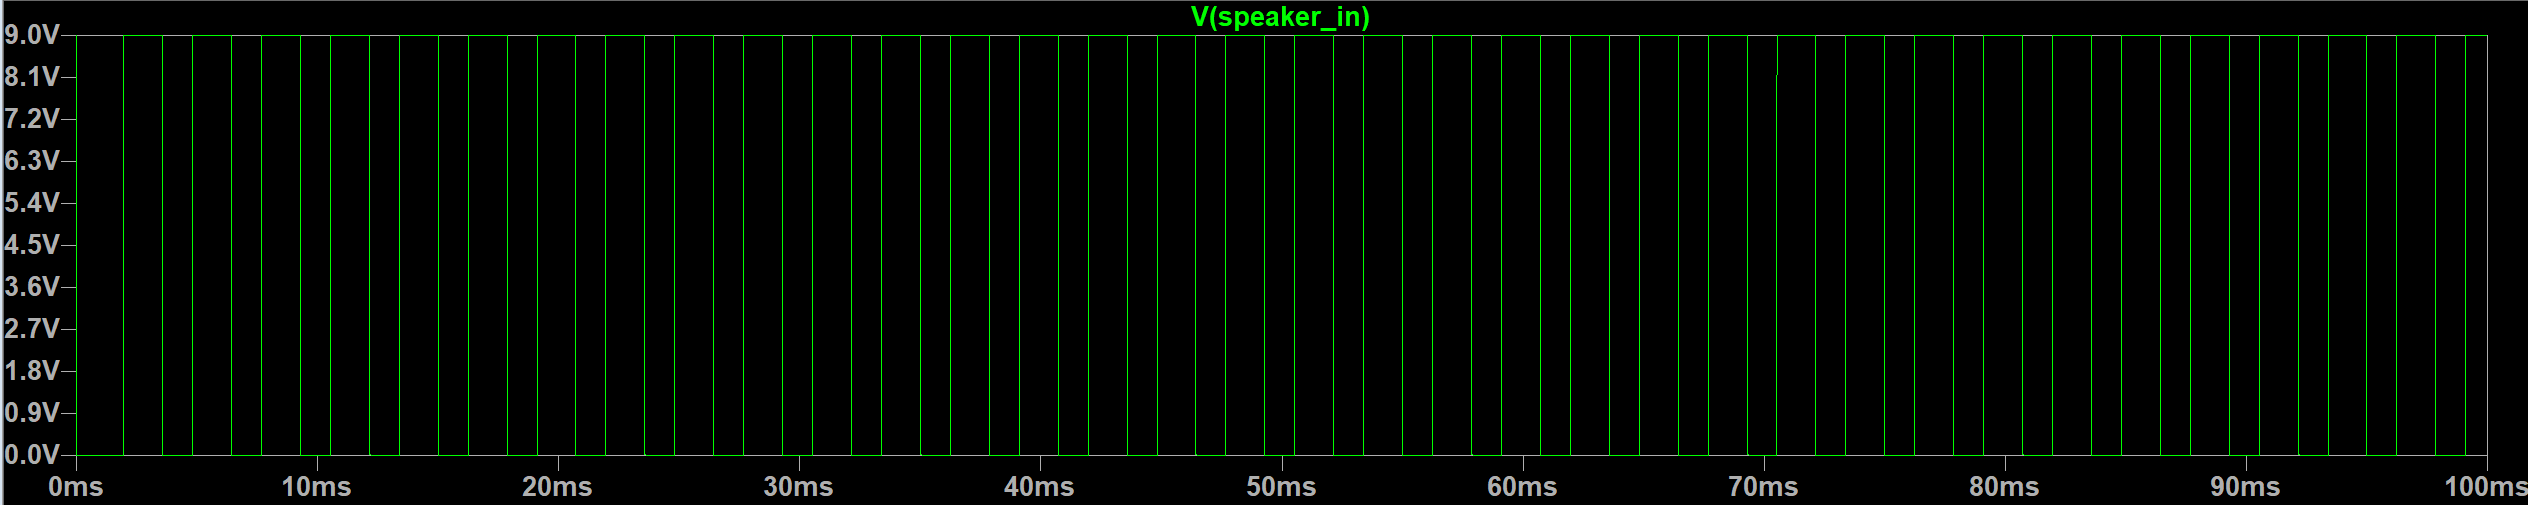
\includegraphics[width=\maxwidth{50.17561465127948em}]{image_10}
\end{flushleft}
\end{par}

\begin{par}
\begin{flushleft}
\textit{[LTSpice Simulation for State 1]}
\end{flushleft}
\end{par}

\begin{par}
\begin{flushleft}
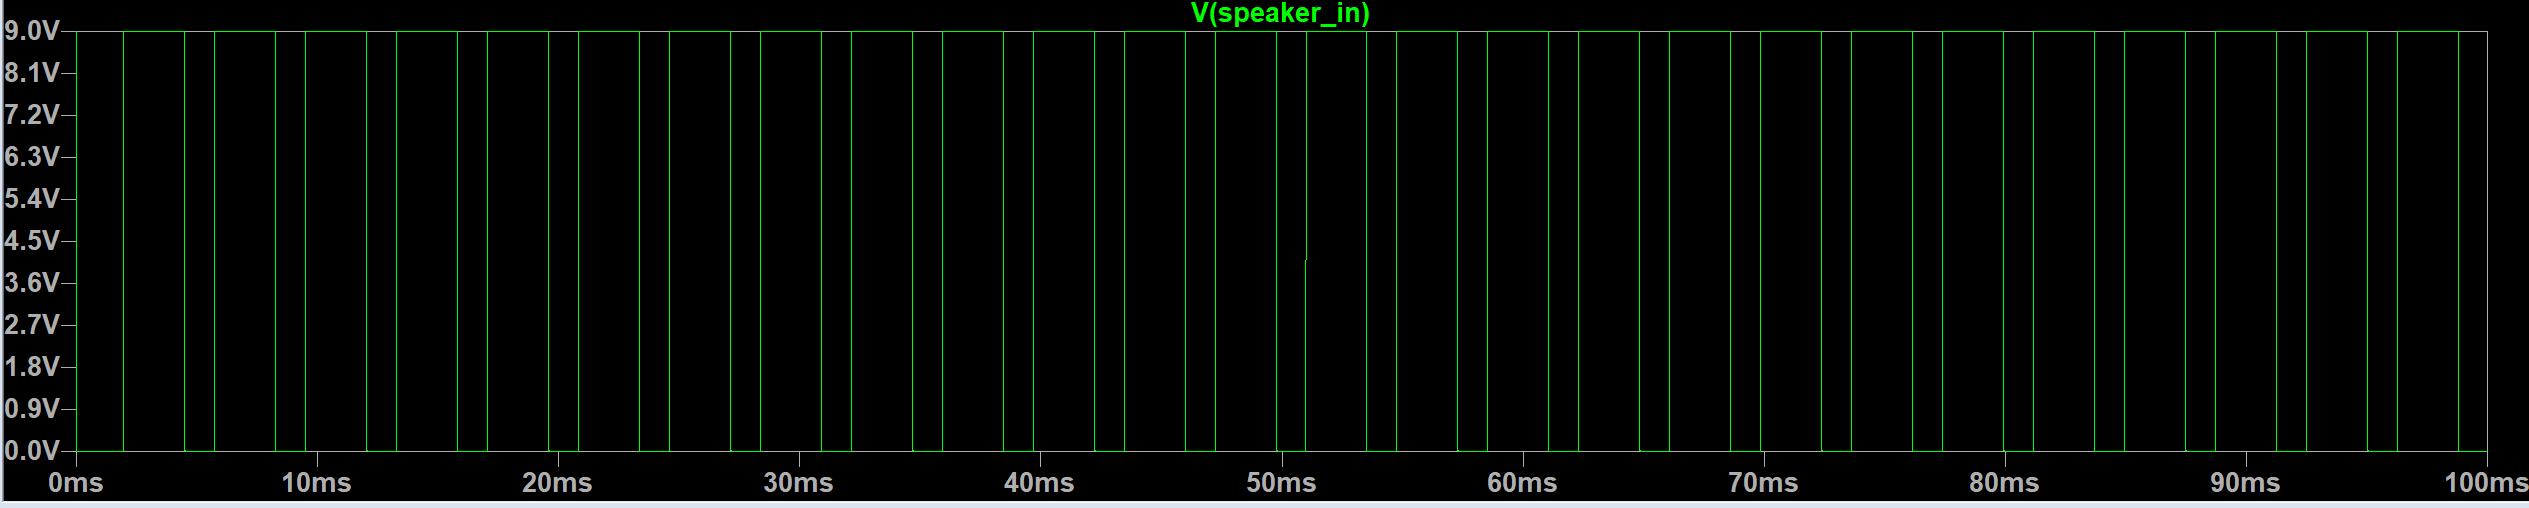
\includegraphics[width=\maxwidth{50.17561465127948em}]{image_11}
\end{flushleft}
\end{par}

\begin{par}
\begin{flushleft}
\textit{[LTSpice Simulation for State 2]}
\end{flushleft}
\end{par}

\begin{par}
\begin{flushleft}
State 1 provides square waves with around 4 oscillations within 10 miliseconds:
\end{flushleft}
\end{par}

\begin{matlabcode}
4/10e-3%frequency
\end{matlabcode}
\begin{matlaboutput}
ans = 400
\end{matlaboutput}

\begin{par}
\begin{flushleft}
State 2 provides square waves with around 3 oscillations within 10 miliseconds:
\end{flushleft}
\end{par}

\begin{matlabcode}
3/10e-3%frequency
\end{matlabcode}
\begin{matlaboutput}
ans = 300
\end{matlaboutput}

\begin{par}
\begin{flushleft}
The estimated calculations of frequency from waveform match with our analytical predictions. 
\end{flushleft}
\end{par}

\label{H_2F6DB34F}
\matlabheadingthree{2.1.5 Test cases}

\begin{par}
\begin{flushleft}
Since this is a direct-current system with almost no configurable parameters, the simulation mentioned above would suffice. 
\end{flushleft}
\end{par}

\begin{par}
\begin{flushleft}
No extra test cases are necessary. 
\end{flushleft}
\end{par}

\label{H_1F280B86}
\matlabheadingtwo{2.2 Physical Electronics/Breadboard Verifications}

\label{H_0CE80909}
\matlabheadingthree{2.2.1 Verified Parts of Design }

\begin{par}
\begin{flushleft}
The entire circuitray is built on breadboard for a through verifications, since the design it not complicated and takes no time to set up. 
\end{flushleft}
\end{par}

\begin{par}
\begin{flushleft}
Thus no simiplications are made.
\end{flushleft}
\end{par}

\label{H_240BCB2D}
\matlabheadingthree{2.2.2 Schematics and Setups}

\begin{par}
\begin{flushleft}
Here is the mapping of components from breadboard to the final PCB board.
\end{flushleft}
\end{par}

\begin{par}
\begin{flushleft}
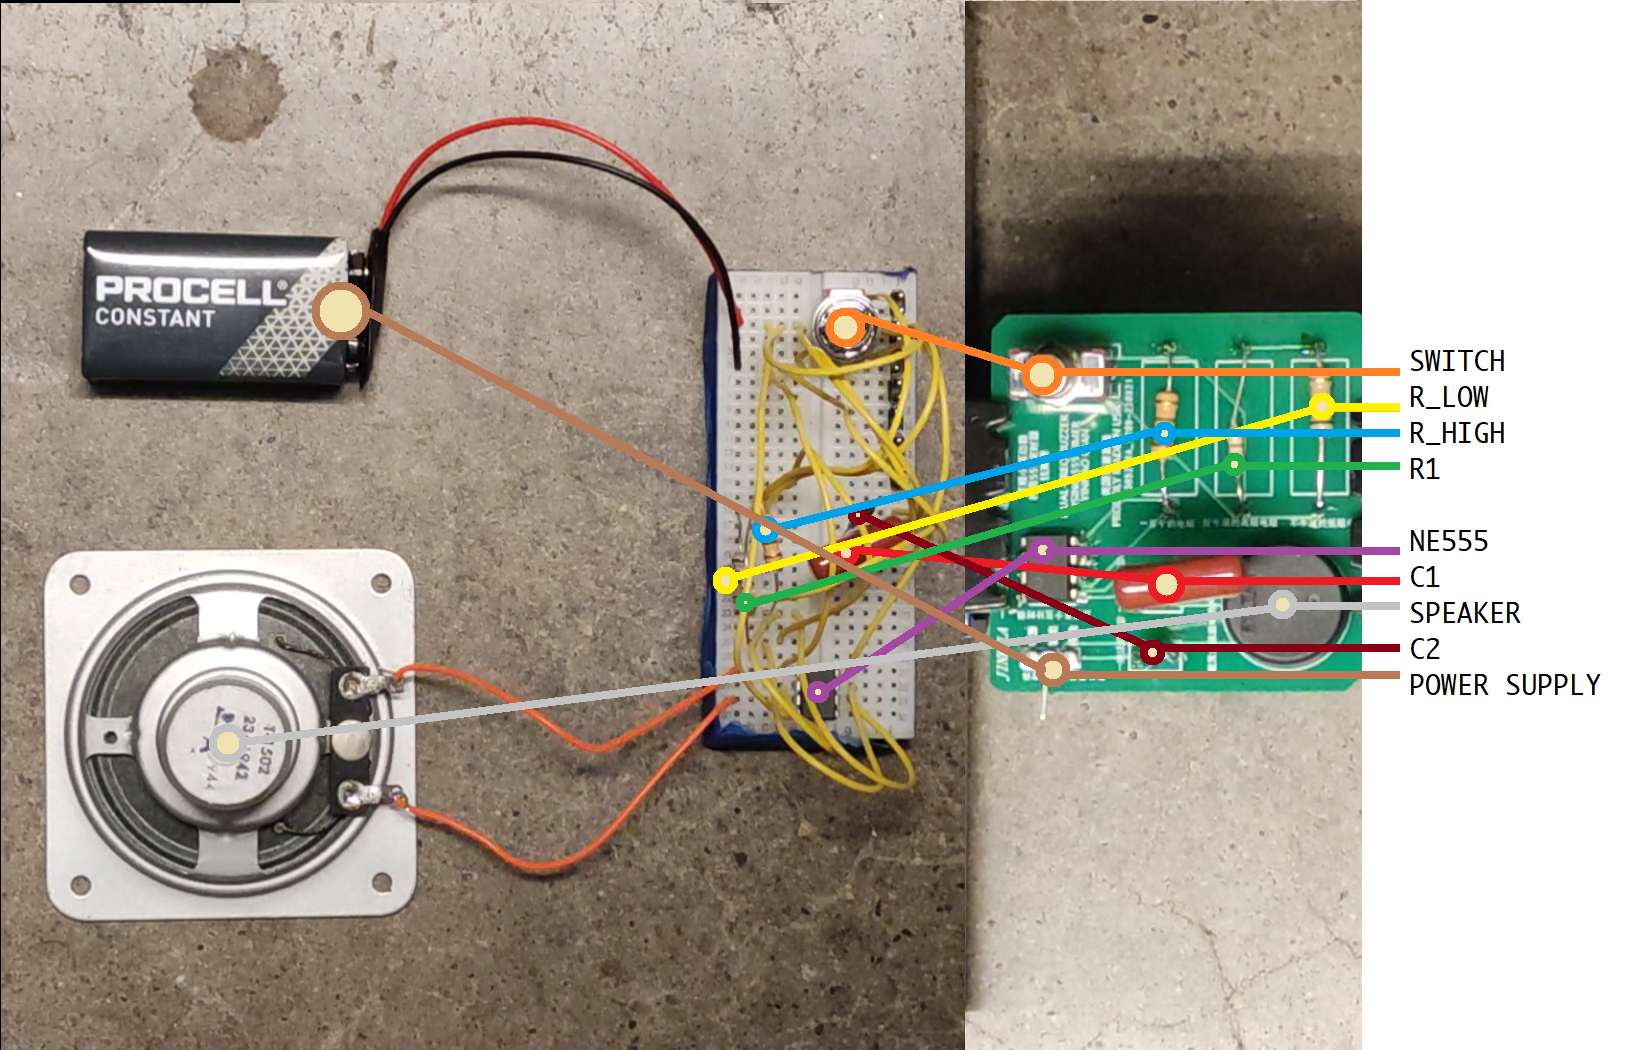
\includegraphics[width=\maxwidth{50.17561465127948em}]{image_12}
\end{flushleft}
\end{par}

\begin{par}
\begin{flushleft}
\textit{[Breadboard and PCB mapping]}
\end{flushleft}
\end{par}

\label{H_50B38FF4}
\matlabheadingthree{2.2.3 Electronic Test Equipments Used}

\begin{par}
\begin{flushleft}
The only dangling parts outside of the breadbaord are the 9-V portable battery and the external speaker. 
\end{flushleft}
\end{par}

\begin{par}
\begin{flushleft}
There is no need to monitor the output voltage using an actual oscilloscope, since the speaker can acts as the "visual oscilloscope", and the volume and tone of sound that the speaker generates dictates the output voltage and frequency.
\end{flushleft}
\end{par}

\label{H_9E5FE4CA}
\matlabheadingthree{2.2.4 Test Cases}

\begin{par}
\begin{flushleft}
Three modes of operations are tested as 3 positions of the switch are togglable:
\end{flushleft}
\end{par}

\begin{itemize}
\setlength{\itemsep}{-1ex}
   \item{\begin{flushleft} Top Position: High Frequency Sound \end{flushleft}}
   \item{\begin{flushleft} Middle Position: No Sound \end{flushleft}}
   \item{\begin{flushleft} Bottom Position: Low Frequency Sound \end{flushleft}}
\end{itemize}

\begin{par}
\begin{flushleft}
All test cases were passed. 
\end{flushleft}
\end{par}

\begin{par}
\begin{flushleft}
No sound information is presentable in this report, and more information is available in the video demostration.
\end{flushleft}
\end{par}


\label{H_954FF7CD}
\matlabheading{3 Design Implementation}

\label{H_B0D033DD}
\matlabheadingtwo{3.1 PCB Design Description}

\label{H_1057BFCE}
\matlabheadingthree{3.1.1 Components Descriptions}

\begin{par}
\begin{flushleft}
The only difference between this PCB schematics and the refereced design schematics is the output voltage pin, and the purpose of this pin is solely for debugging purposes, and should not be used during normal operations. 
\end{flushleft}
\end{par}

\begin{par}
\begin{flushleft}
All remaining components are the same. 
\end{flushleft}
\end{par}

\begin{par}
\begin{flushleft}
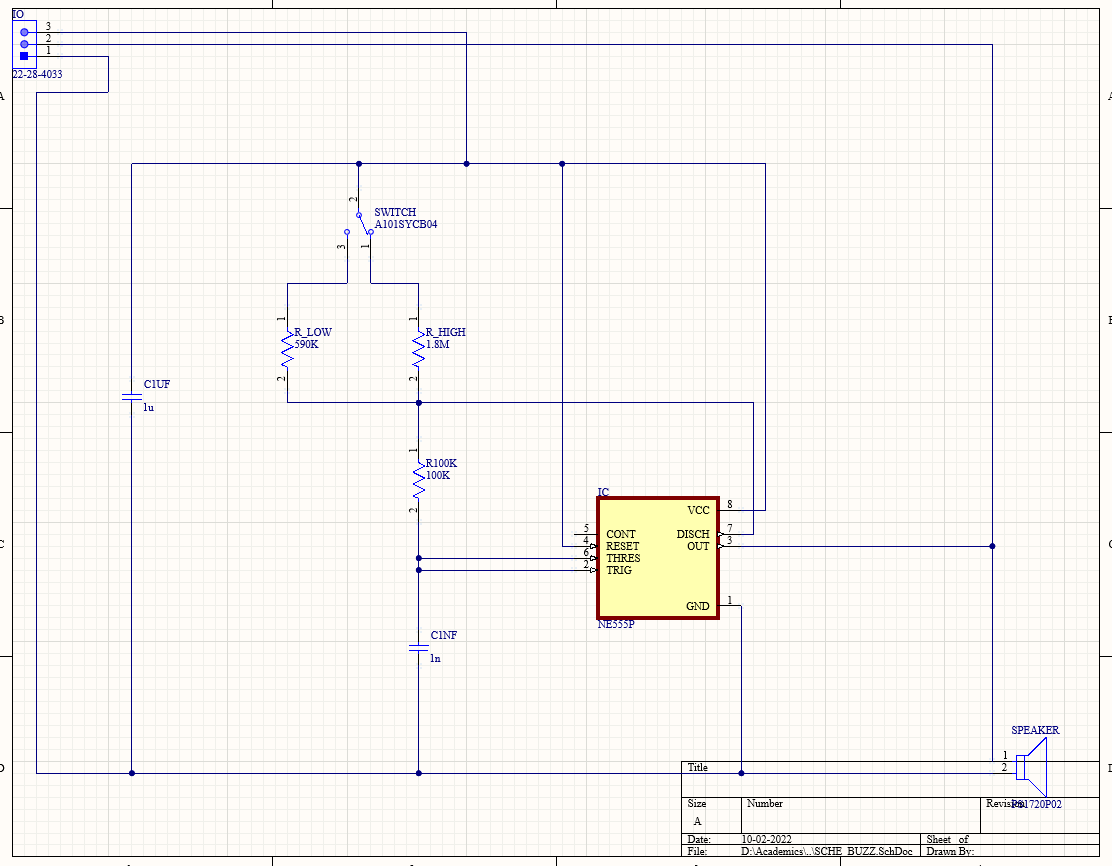
\includegraphics[width=\maxwidth{50.17561465127948em}]{image_13}
\end{flushleft}
\end{par}

\begin{par}
\begin{flushleft}
\textit{[PCB Schematics in Altium]}
\end{flushleft}
\end{par}

\label{H_A54699DF}
\matlabheadingthree{3.1.2 Components Usages Descriptions}

\begin{par}
\begin{flushleft}
All resistors and capacitors are through-hole instead of surface-mount. 
\end{flushleft}
\end{par}

\begin{par}
\begin{flushleft}
The original design includes surface-mount components, yet the final design replaced all to through-hole ones, as surface-mount components is siginificantly smaller in size, and higher in installation efforts; surface-mount components are unavilable in Benedum Hall. 
\end{flushleft}
\end{par}

\begin{par}
\begin{flushleft}
The three-pin header reduces the effort to connect the power source and ground to the PCB board: this versatile interface allows the user to decide what catagories of power supply (battery, waveform generator, power adaptor) to avail. 
\end{flushleft}
\end{par}

\label{H_93279166}
\matlabheadingtwo{3.2 PCB Layout}

\label{H_CF112E74}
\matlabheadingthree{3.2.1 Overview}

\begin{par}
\begin{flushleft}
On the left is the layout preview while on the right is the final production preview. 
\end{flushleft}
\end{par}

\begin{par}
\begin{flushleft}
Components are arranged in a way so that minimal board area is used; this design is compact, and no space is wasted at all. 
\end{flushleft}
\end{par}

\begin{par}
\begin{flushleft}
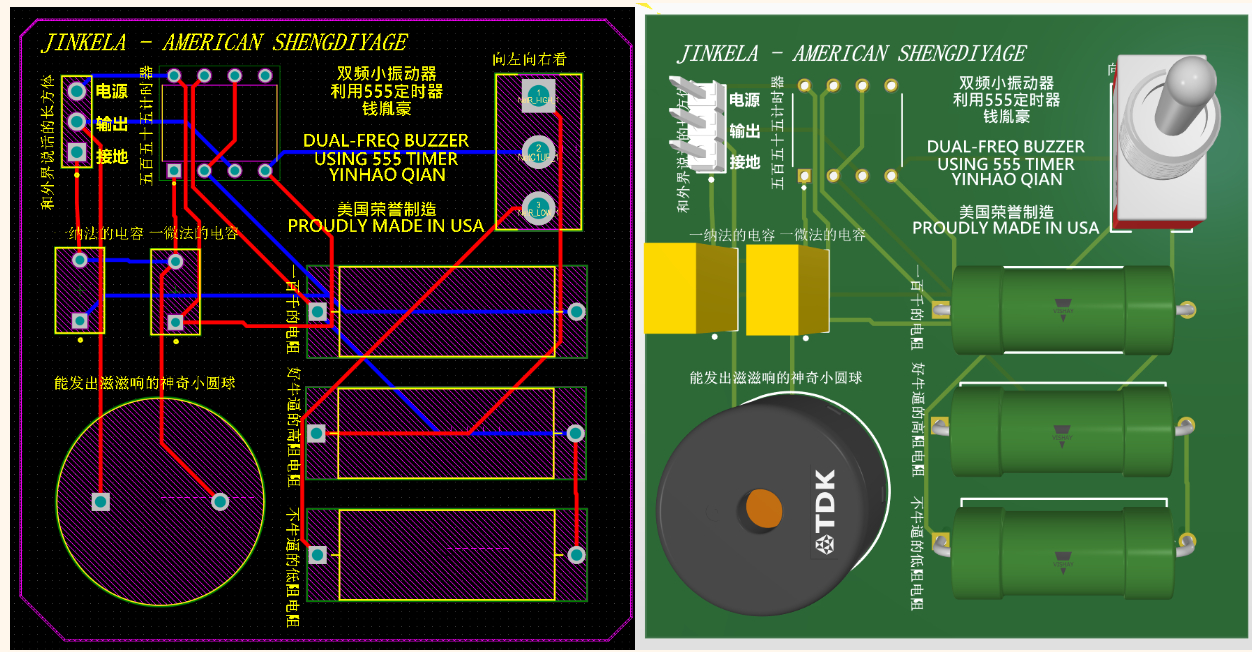
\includegraphics[width=\maxwidth{50.17561465127948em}]{image_14}
\end{flushleft}
\end{par}

\begin{par}
\begin{flushleft}
\textit{[PCB Layout in Altium]}
\end{flushleft}
\end{par}

\label{H_61C1F921}
\matlabheadingthree{3.2.2 Components Packaging}

\begin{par}
\begin{flushleft}
Mentioned from previous sections, all surface-mount resistors and capacitors, which are included in the first version of blueprint, are all replaced with their through-hole counterparts for easier installation purposes. 
\end{flushleft}
\end{par}

\label{H_B09F4655}
\matlabheadingthree{3.2.3 Best Practices}

\begin{par}
\begin{flushleft}
One of the key of reducing the cost of board production is using a square board layout rather than a rectangular board layout, as the cost of production depends on the maximum side length of board. 
\end{flushleft}
\end{par}

\begin{par}
\begin{flushleft}
Additionally, all input and output ports are marked with clear names in local language, as mistakenly reversing the polarity will damage the circuit and result in undefined electrical behaviors.
\end{flushleft}
\end{par}

\label{H_82BB6459}
\matlabheadingthree{3.2.4 Design Processes}

\begin{par}
\begin{flushleft}
Similar components are placed next to each others: capacitors and resistors are placed in groups for easy catagorization.
\end{flushleft}
\end{par}

\begin{par}
\begin{flushleft}
Input and output pins are placed at the board corner so that users are able to sort the connections in order. 
\end{flushleft}
\end{par}

\begin{par}
\begin{flushleft}
No challanges are present in the design process since directions are clear and comprehensible. 
\end{flushleft}
\end{par}

\begin{par}
\begin{flushleft}
Circuit schematics produced no errors. Rule files are imported accordingly and produced zero errors on the first attempt of rule checks. 
\end{flushleft}
\end{par}

\begin{par}
\begin{flushleft}
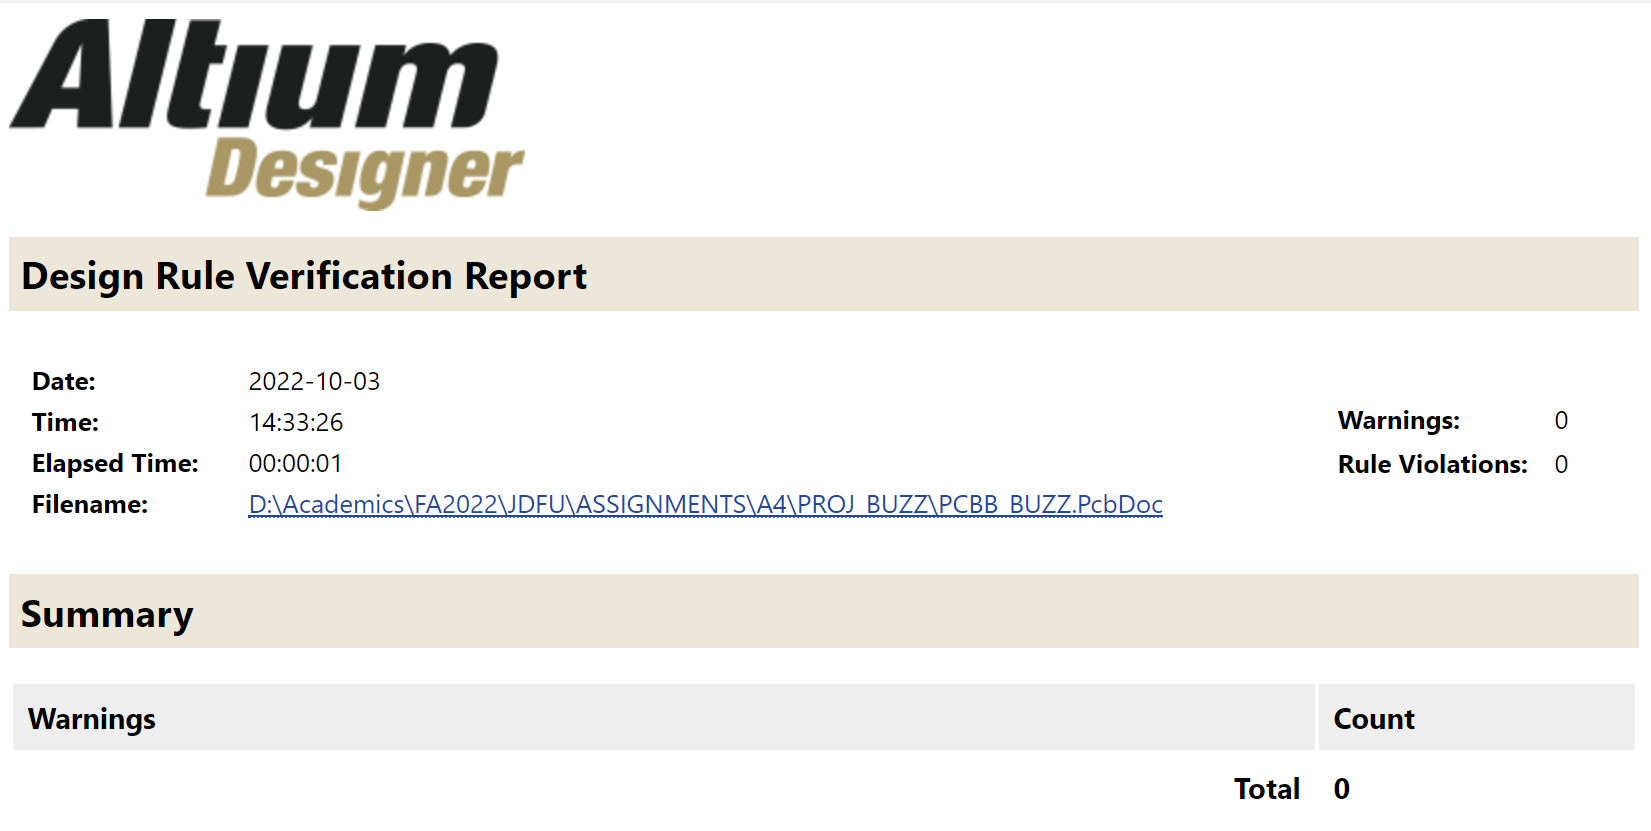
\includegraphics[width=\maxwidth{50.17561465127948em}]{image_15}
\end{flushleft}
\end{par}

\begin{par}
\begin{flushleft}
\textit{[Rule Checks on Altium]}
\end{flushleft}
\end{par}

\begin{par}
\begin{flushleft}
No layout changes are made throughout the designing process.
\end{flushleft}
\end{par}


\label{H_C1F13D1A}
\matlabheading{4 Design Manufacturing and Assembly}

\label{H_2B8380E8}
\matlabheadingtwo{4.1 Soldering and Assembling Approach}

\begin{par}
\begin{flushleft}
The PCB board is soldered using a circuit board holder, lead solder, a soldering iron, and a solder smoke absorber.
\end{flushleft}
\end{par}

\begin{par}
\begin{flushleft}
Solder is applied next to the hot soldering iron while the iron is touching the pins of components. Solder is then melted on angular rings and flowed through vias, forming a strong bond between the components and rings from both top and bottom layers. 
\end{flushleft}
\end{par}

\label{H_1983111B}
\matlabheadingtwo{4.2 Soldering Methods Used}

\begin{par}
\begin{flushleft}
The same soldering techniques are used from the instruction videos mentioned during lecture times. 
\end{flushleft}
\end{par}

\begin{par}
\begin{flushleft}
For safety reasons, goggles and insulating gloves are used as well. 
\end{flushleft}
\end{par}

\begin{par}
\begin{flushleft}
To ensure the durability, more solder is applied to the board comparing to the standard.
\end{flushleft}
\end{par}

\begin{par}
\begin{flushleft}
Flux is subsequently cleaned, although debris cannot be fully removed. 
\end{flushleft}
\end{par}

\label{H_E3415F9F}
\matlabheadingtwo{4.3 Soldering Challanges}

\begin{par}
\begin{flushleft}
The head of soldering iron is oxidized and masked with undesired insulating layers. 
\end{flushleft}
\end{par}

\begin{par}
\begin{flushleft}
Attempts to remove the layers are conducted yet unsucessful, and it takes more than five seconds to melt the lead-free solder; to amelirate this issue, lead solder is used as they have relatively lower melting points. 
\end{flushleft}
\end{par}

\begin{par}
\begin{flushleft}
No modifications are made for testing. 
\end{flushleft}
\end{par}


\label{H_D26F16D2}
\matlabheading{5 Design Testing}

\label{H_331FD6BD}
\matlabheadingtwo{5.1 Test Plans}

\begin{par}
\begin{flushleft}
Two means of tests are conducted: voltage monitoring method and sound monitoring method.
\end{flushleft}
\end{par}

\begin{par}
\begin{flushleft}
First, the output voltage will be monitored and recorded using a oscilloscope from the output voltage debugging pin (the middle pin) while toggling the switch to three positions.
\end{flushleft}
\end{par}

\begin{par}
\begin{flushleft}
Second, the sound output from buzzer will be heard and evaluated while toggling the switch to three positions, and this part is shown in the video demostration.
\end{flushleft}
\end{par}

\label{H_48183751}
\matlabheadingtwo{5.2 Assembled Prototypes and Test Results}

\begin{par}
\begin{flushleft}
Below are the fully assembled and functional prototypes for both PCB and breadboard.
\end{flushleft}
\end{par}

\begin{par}
\begin{flushleft}
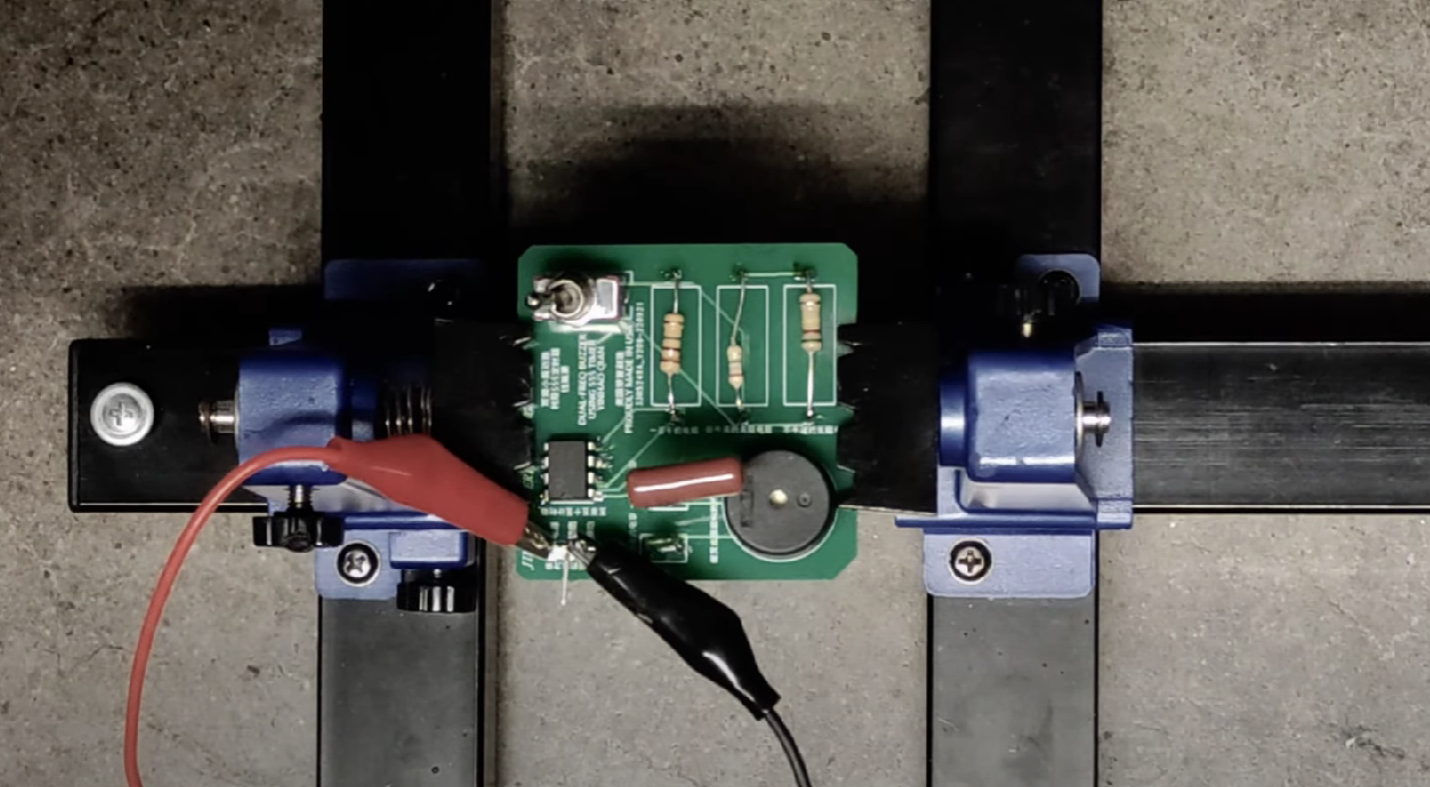
\includegraphics[width=\maxwidth{50.17561465127948em}]{image_16}
\end{flushleft}
\end{par}

\begin{par}
\begin{flushleft}
\textit{[Assembled PCB Board Prototype]}
\end{flushleft}
\end{par}

\begin{par}
\begin{flushleft}
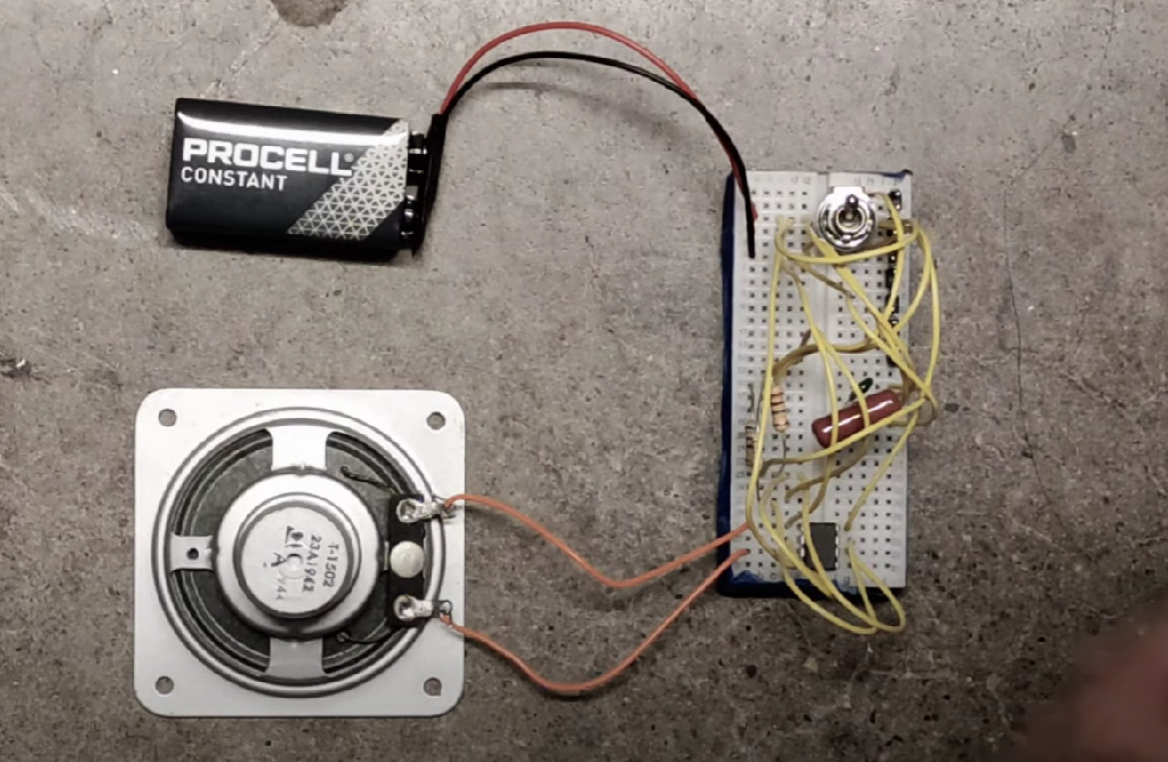
\includegraphics[width=\maxwidth{50.17561465127948em}]{image_17}
\end{flushleft}
\end{par}

\begin{par}
\begin{flushleft}
\textit{[Assembled Breadboard Prototype]}
\end{flushleft}
\end{par}

\begin{par}
\begin{flushleft}
Voltage output can be monitored and recorded at ease with the use of ADALM2000 learning module; analog Channel 1+ and 1- are each connected to OUTPUT pin and GND pin accordingly.
\end{flushleft}
\end{par}

\begin{par}
\begin{flushleft}
While the switch is toggled to top position, a square wave with relatively high frequency is detected at output pin: 
\end{flushleft}
\end{par}

\begin{par}
\begin{flushleft}
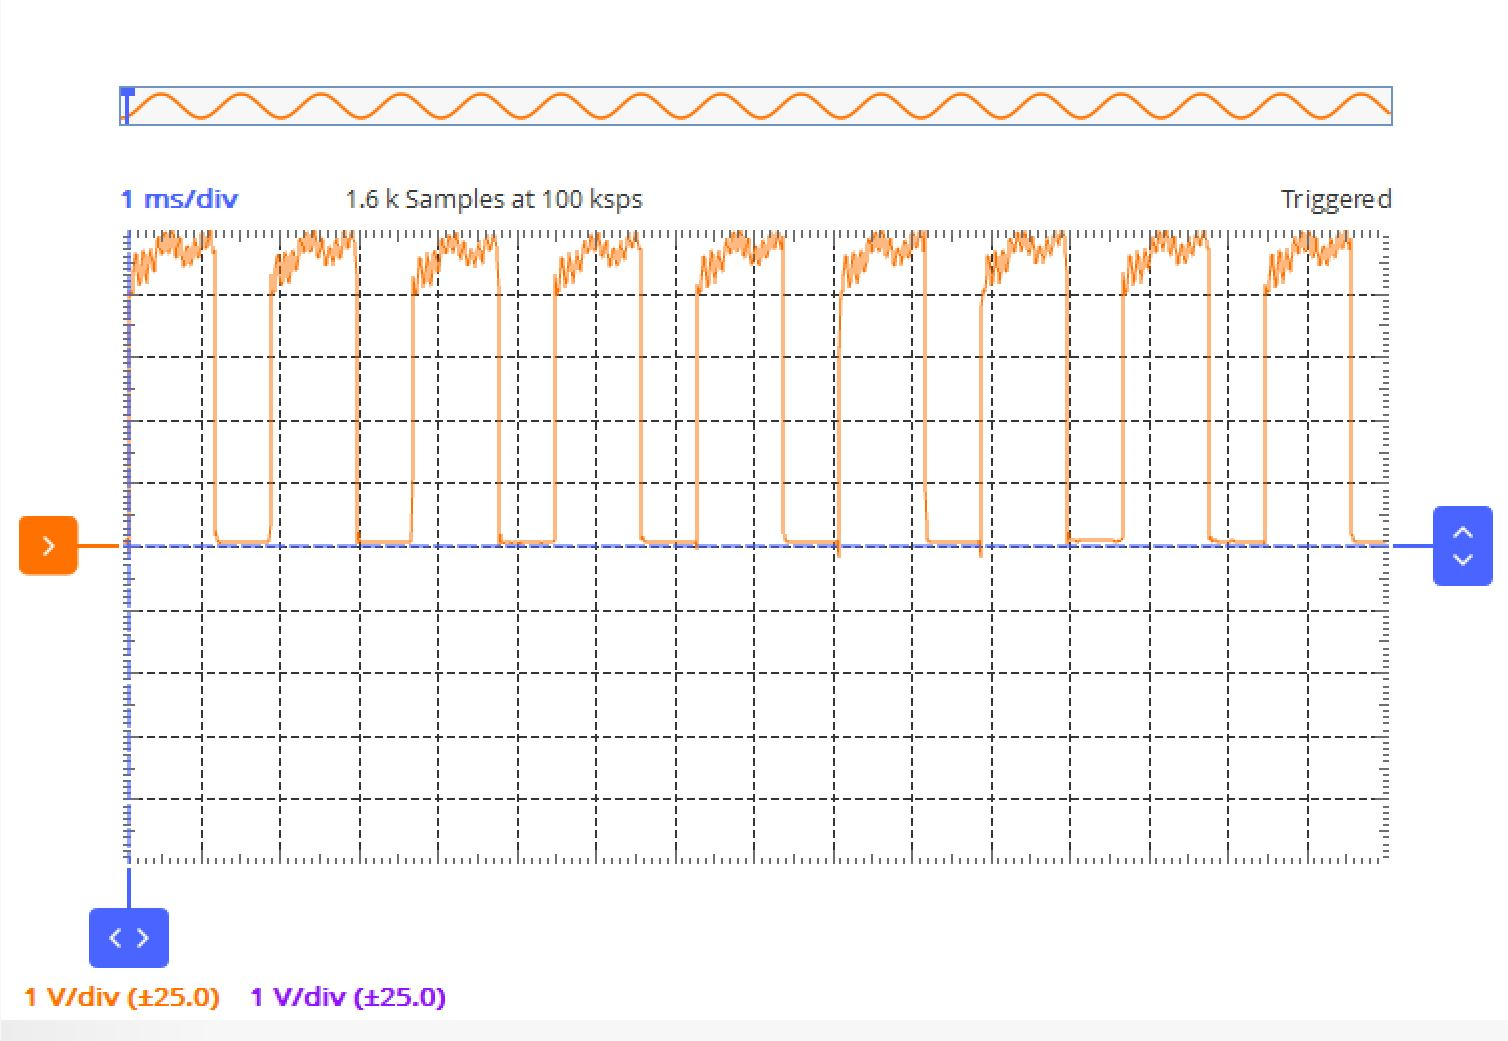
\includegraphics[width=\maxwidth{50.17561465127948em}]{image_18}
\end{flushleft}
\end{par}

\begin{par}
\begin{flushleft}
\textit{[Voltage recorded at high frequency sound mode]}
\end{flushleft}
\end{par}

\begin{par}
\begin{flushleft}
While the switch is toggled to bottom position, a square wave with relatively low frequency is detected at output pin: 
\end{flushleft}
\end{par}

\begin{par}
\begin{flushleft}
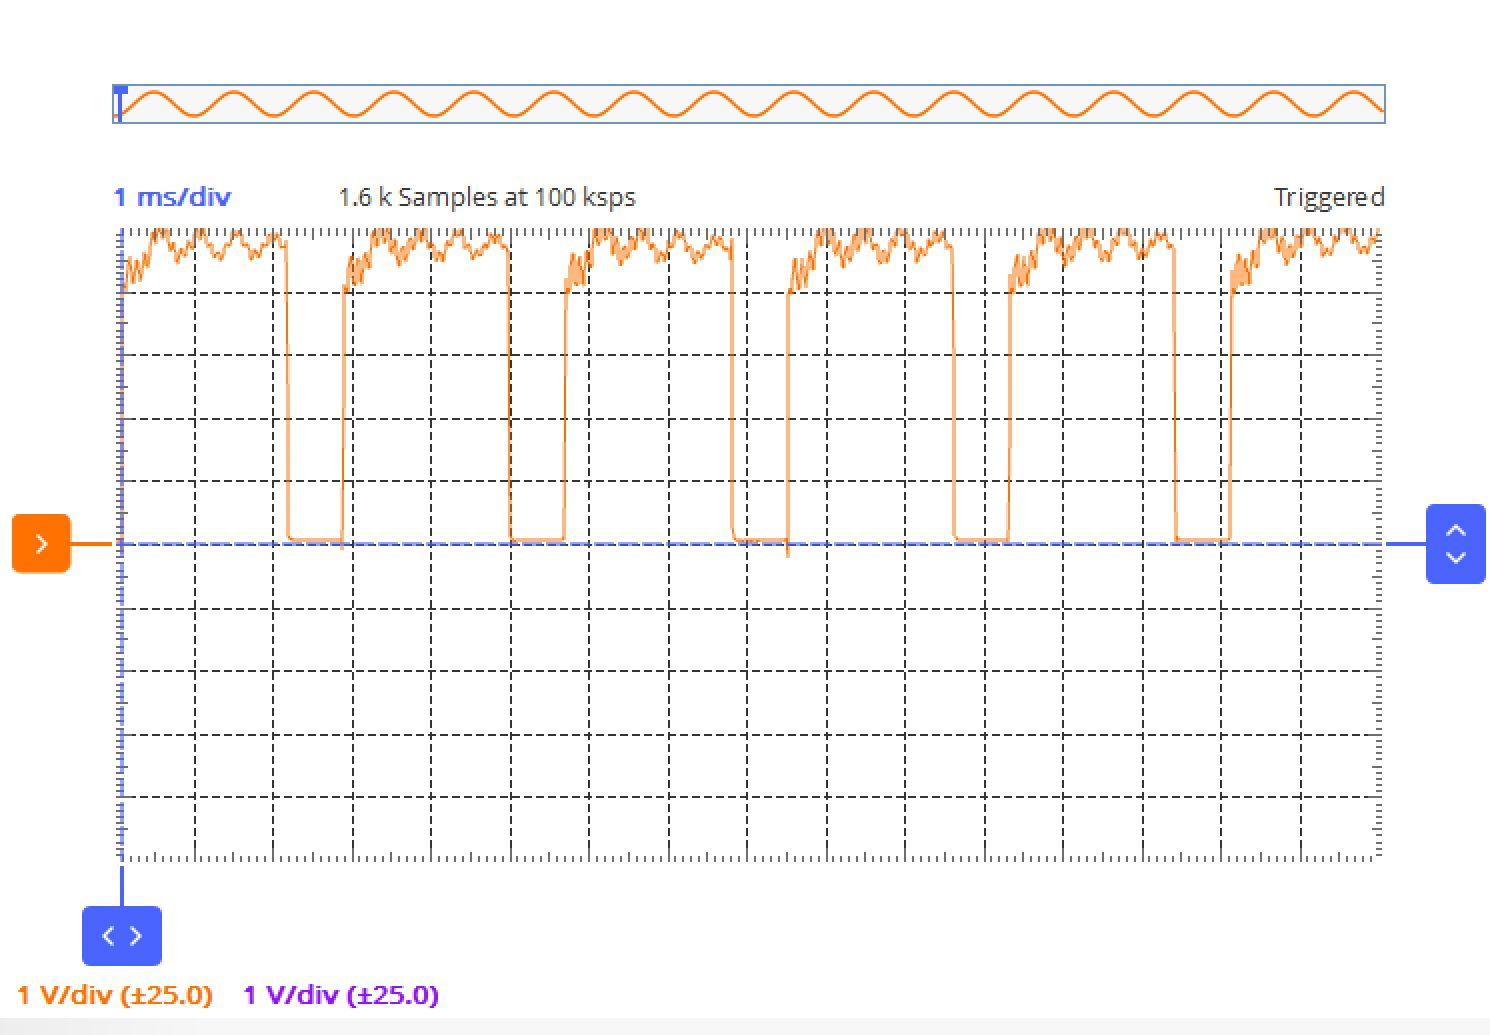
\includegraphics[width=\maxwidth{50.17561465127948em}]{image_19}
\end{flushleft}
\end{par}

\begin{par}
\begin{flushleft}
\textit{[Voltage recorded at low frequency sound mode]}
\end{flushleft}
\end{par}

\begin{par}
\begin{flushleft}
Interestingly, the time low is held constant across both cases, and the time high is varied.
\end{flushleft}
\end{par}

\begin{par}
\begin{flushleft}
This is a predicted behavior as $\textrm{R2}$, the sole dependable resistor of time low, is constant.
\end{flushleft}
\end{par}

\begin{par}
\begin{flushleft}
However, sound test cannot be shown clearly in photo, so please refer to the video demostration to hear the generated sound in both frequencies of sound.
\end{flushleft}
\end{par}

\label{H_72BF1D0C}
\matlabheadingtwo{5.3 Unsucessful Attempts}

\begin{par}
\begin{flushleft}
There is no unsucessful attempts. Both the PCB and breadboard prototypes function as expected on the first trial.
\end{flushleft}
\end{par}

\label{H_AD199618}
\matlabheadingtwo{5.4 Debugging Processes}

\begin{par}
\begin{flushleft}
Since there is no unsucessful attempts, no debugging is needed.
\end{flushleft}
\end{par}

\label{H_3E504880}
\matlabheadingtwo{5.5 Video Demostration Reference}

\begin{par}
\begin{flushleft}
Video demostration is uploaded to Youtube and is now set to public.
\end{flushleft}
\end{par}

\begin{par}
\begin{flushleft}
Both breadboard showcase and PCB board showcase is included in this one video:
\end{flushleft}
\end{par}

\begin{par}
\begin{flushleft}
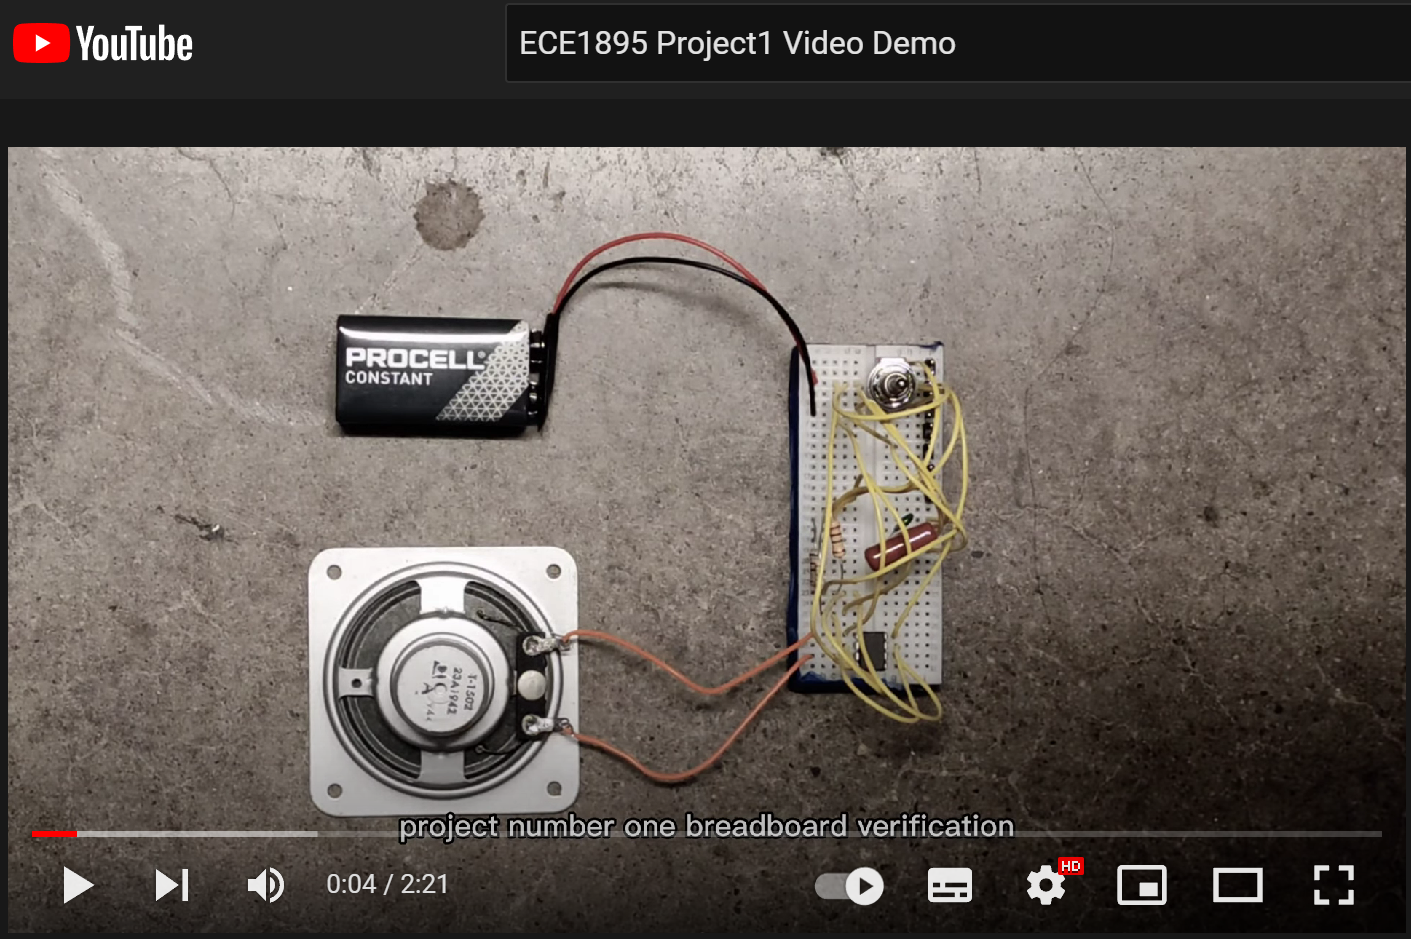
\includegraphics[width=\maxwidth{50.17561465127948em}]{image_20}
\end{flushleft}
\end{par}

\begin{par}
\begin{flushleft}
\textit{[Video Demostration] }\href{https://youtu.be/7KIgePU9fTM}{\textit{https://youtu.be/7KIgePU9fTM}}
\end{flushleft}
\end{par}

\end{document}
